% Praca magisterska - Michał Cichoń, AGH 2014
% Title: Silnik do automatycznej kategoryzacji obrazów
\documentclass[a4paper,12pt]{book}
\usepackage[utf8]{inputenc}
\usepackage[T1]{polski}
\usepackage{polski}
\usepackage{color}
\usepackage{helvet}
\usepackage{graphicx}
\usepackage{times}
\usepackage{geometry}
\usepackage{epstopdf}
\usepackage{titlesec}
\usepackage{indentfirst}
\usepackage{verbatim}
\usepackage{moreverb}
\usepackage{nameref}
\usepackage{listings}
\usepackage{paralist}
\usepackage{amsmath}
\usepackage{url}
\usepackage[font=footnotesize,labelfont=bf]{caption}
\geometry{hmargin={2cm, 2cm}, height=10.0in}
\assignpagestyle{\chapter}{empty}
\linespread{1.3} %interlinia ustawiona na 1.5; 1.3 (LaTeX) to 1.5, 1.6 (LaTeX) to 2

\newcommand{\highlight}[1]{\colorbox{yellow}{#1}}

\newenvironment{dedication}
{
   \cleardoublepage
   \thispagestyle{empty}
   \vspace*{\stretch{10}}
   \hfill\begin{minipage}[t]{0.66\textwidth}
   \raggedright
}%
{
   \end{minipage}
   \vspace*{\stretch{3}}
   \clearpage
}

\begin{document}
\nocite{*}

% =====  STRONA TYTULOWA PRACY MAGISTERSKIEJKIEJ ====
% ostatnia modyfikacja: 2009/07/01, K. Malarz

\thispagestyle{empty}
%% ------------------------ NAGLOWEK STRONY ---------------------------------

\includegraphics[height=37.5mm]{agh_nzw_a_pl_1w_wbr_cmyk.eps}\\
\rule{30mm}{0pt}
{\large \textsf{Wydział Fizyki i Informatyki Stosowanej}}\\
\rule{\textwidth}{3pt}\\
\rule[2ex]
{\textwidth}{1pt}\\
\vspace{6ex}
\begin{center}
{\LARGE \bf \textsf{Praca magisterska}}\\
\vspace{13ex}
% --------------------------- IMIE I NAZWISKO -------------------------------
{\bf \Large \textsf{Michał Cichoń}}\\
\vspace{3ex}
{\sf\small kierunek studiów:} {\bf\small \textsf{informatyka stosowana}}\\
\vspace{1.5ex}
{\sf\small specjalność:} {\bf\small \textsf{grafika komputerowa i przetwarzanie obrazów}}\\
\vspace{10ex}
%% ------------------------ TYTUL PRACY --------------------------------------
{\bf \huge \textsf{Silnik do automatycznej kategoryzacji obrazów}}\\
\vspace{14ex}
%% ------------------------ OPIEKUN PRACY ------------------------------------
{\Large Opiekun: \bf \textsf{dr inż.\ Maciej Śniechowski}}\\
\vspace{22ex}
{\large \bf \textsf{Kraków, wrzesień 2014}}
\end{center}
%% =====  STRONA TYTUŁOWA PRACY MAGISTERSKIEJKIEJ ====

\newpage

%% =====  TYŁ STRONY TYTUŁOWEJ PRACY MAGISTERSKIEJKIEJ ====
{\sf Oświadczam, świadomy odpowiedzialności karnej za poświadczenie nieprawdy, że niniejszą pracę dyplomową wykonałem osobiście i samodzielnie i  nie korzystałem ze źródeł innych niż wymienione w pracy.}

\vspace{14ex}

\begin{center}
\begin{tabular}{lr}
~~~~~~~~~~~~~~~~~~~~~~~~~~~~~~~~~~~~~~~~~~~~~~~~~~~~~~~~~~~~~~~~~ &
................................................................. \\
~ & {\sf (czytelny podpis)}\\
\end{tabular}
\end{center}

%% =====  TYL STRONY TYTULOWEJ PRACY MAGISTERSKIEJKIEJ ====

\newpage
\rightline{Kraków, .....................}
\begin{center}
{\bf Tematyka pracy magisterskiej i praktyki dyplomowej
Michała Cichonia,
studenta V roku studiów kierunku informatyka stosowana, specjalności grafika komputerowa i przetwarzanie obrazów.}\\
\end{center}

Temat pracy magisterskiej:
{\bf Silnik do automatycznej kategoryzacji obrazów}\\

\begin{tabular}{rl}

Opiekun pracy:                  & dr inż.\ Maciej Śniechowski\\
Recenzenci pracy:               & ...\\
Miejsce praktyki dyplomowej:    & WFiIS AGH, Kraków\\
\end{tabular}

\begin{center}
{\bf Program pracy magisterskiej i praktyki dyplomowej}
\end{center}

\begin{enumerate}
\item Omówienie realizacji pracy magisterskiej z opiekunem.
\item Praktyka dyplomowa:
\begin{itemize}
\item zebranie i opracowanie literatury dotyczącej tematu pracy.
\item zebranie zbioru zdjęć treningowych.
\item sporządzenie sprawozdania z praktyki.
\end{itemize}
\item Stworzenie silnika kategoryzacyjnego.
\item Zebranie i opracowanie wyników.
\item Analiza wyników, ich omówienie i zatwierdzenie przez opiekuna.
\item Opracowanie redakcyjne pracy.
\end{enumerate}


\noindent
Termin oddania w dziekanacie: .....................\\[1cm]

\begin{center}
\begin{tabular}{lcr}
.............................................................. & ~~~ &
.............................................................. \\
(podpis kierownika katedry) & & (podpis opiekuna) \\
\end{tabular}
\end{center}

\newpage

\noindent
Na kolejnych dwóch stronach proszę dołączyć kolejno recenzje pracy popełnione przez Opiekuna oraz Recenzenta (wydrukowane z systemu MISIO i podpisane przez odpowiednio Opiekuna i Recenzenta pracy). Papierową wersję pracy (zawierającą podpisane recenzje) proszę złożyć w dziekanacie celem rejestracji co najmniej na tydzień przed planowaną obroną.

\newpage

\noindent
Na kolejnych dwóch stronach proszę dołączyć kolejno recenzje pracy popełnione przez Opiekuna oraz Recenzenta (wydrukowane z systemu MISIO i podpisane przez odpowiednio Opiekuna i Recenzenta pracy). Papierową wersję pracy (zawierającą podpisane recenzje) proszę złożyć w dziekanacie celem rejestracji co najmniej na tydzień przed planowaną obroną.

%TODO DODAĆ PODZIĘKOWANIA
\begin{dedication}
\textit{Chciałbym złożyć serdeczne podziękowania...}
\end{dedication}

\tableofcontents

\setlength{\parskip}{1ex plus 0.5ex minus 0.2ex}

\chapter*{Wstęp}

%TODO TEN WSTEP WYMAGA POPRAWEK
\addcontentsline{toc}{chapter}{Wstęp}
Jednym z największych wyzwań, przed którymi stoi współczesna informatyka, jest przetwarzanie dużych ilości danych. Coraz częściej dane te nie reprezentują informacji liczbowych lub tekstowych, ale zawierają pewien rodzaj obrazu. 

Dobrą ilustracją tego zjawiska jest przykład przeglądarki internetowej Google, gdzie początkowo kładziony był nacisk na wyszukiwanie danych tekstowych, a obecnie obrazy są bardzo dynamicznie rozwijanym zasobem, którego indeksowanie w latach 2001-2010 zwiększyło się z 250 mln do ponad 10 mld.\cite{Google2010} 

Obrazy cyfrowe mają szereg zastosowań, od bardzo prozaicznych takich jak reprezentacja amatorskich zdjęć wykonanych cyfrowym aparatem fotograficznym, do bardzo zaawansowanych takich jak chociażby diagnostyka medyczna, gdzie informacja zawarta na zdjęciu jest kluczowa i niekiedy decyduje o ludzkim życiu.

Zarządzając dużym zbiorem obrazów często posługujemy się opisem słownym. Opis taki, w~formie nazwy pliku, metadanych EXIF\footnote{EXIF - Exchangeable Image File Format, najpopularniejszy standard metadanych dla plików ze zdjęciami cyfrowymi} lub rekordu w bazie danych, daje nam pewne wyobrażenie o tym co znajduje się na obrazie. Wyobrażenie to może być jednak mylne, lub niedostateczne, by pozwalało nam na poprawne jego zidentyfikowanie.

Pomoc w rozwiązaniu tego problemu daje nam teoria rozpoznawania obrazów, stosunkowo nowa, ale bardzo szybko rozwijająca się gałąź informatyki, która daje nam narzędzia umożliwiające takie przetwarzanie obrazów by możliwe stało się rozpoznanie przynależności obrazu do pewnej klasy.\cite{Tad91}

%TODO NAPISAĆ O CRIB (Wyszukiwanie informacji w dużych zbiorach obrazów)

\section*{Cel pracy}
\addcontentsline{toc}{section}{Cel pracy}

%TODO KONIECZNIE TRZEBA TO ZMIENIĆ - wstęp nieproporcjonalnie za długi w stosunku
%TODO do faktycznego celu pracy, domeny (2) też są nienajlepsze
Stworzenie systemu informatycznego, który pomógłby skategoryzować obrazy na podstawie ich zawartości mogłoby okazać się bardzo pomocne w wielu dziedzinach gospodarki, w których znalezienie odpowiedniej ilustracji do prezentowanych danych jest kluczowe takich jak: biznes, marketing, medycyna.

Celem pracy jest stworzenie silnika kategoryzacyjnego, który na podstawie danych wyekstratowanych z obrazu będzie w stanie przyporządkować obraz do najbardziej odpowiedniej kategorii.

\section*{Przykłady implementacji}
\addcontentsline{toc}{section}{Przykłady implementacji}
Napisać o:

- http://imagga.com/solutions/categorization-api.html

- http://googleblog.blogspot.com/2010/07/ooh-ahh-google-images-presents-nicer.html (problem z tulipanem)
\chapter{Podstawy teoretyczne}

Problem kategoryzacji obrazów wpisuje się w dziedzinę rozpoznawania obrazów. Zadanie to polega na rozpoznaniu przynależności różnych rodzajów obiektów do pewnych klas\cite{Tad91} i jest częścią większego zagadnienia, które określa się jako uczenie maszynowe.

\section{Uczenie maszynowe}

Uczenie maszynowe jest zagadnieniem interdyscyplinarnym z pogranicza informatyki, statystyki i sztucznej inteligencji, które zajmuje się tworzeniem systemów mogących doskonalić się za pomocą dostarczanych danych.

Systemy te ulegają nieustannej modyfikacji, zmieniają swoje wewnętrzne parametry po to by osiągnąć korzyści takie jak zwiększenie efektywności lub wydajności działania. Ważną cechą jest to, że jakkolwiek zmiany te zachodzą na podstawie czynników zewnętrznych to jednak dokonują się w~systemie autonomicznie. System, który się uczy zmienia sam siebie na lepsze.\cite{CICHOSZ00}

\section{Uczenie nadzorowane i nienadzorowane}

W uczeniu maszynowym możemy wyróżnić dwa zasadnicze podejścia: uczenie nadzorowane (\emph{ang. supervised machine learning}) i nienadzorowane (\emph{ang. unsupervised machine learning}). Różnica pomiędzy nimi polega na obecności w uczeniu nadzorowanym tzw. nauczyciela, który stanowi źródło informacji trenującej. Posługując się analogiczną terminologią, system który podlega nauce określa się jako ucznia. Na rys. \ref{fig:supervised-learning} przedstawiono schemat uczenia maszynowego z użyciem nauczyciela.

\begin{figure}[h]
	\centering
	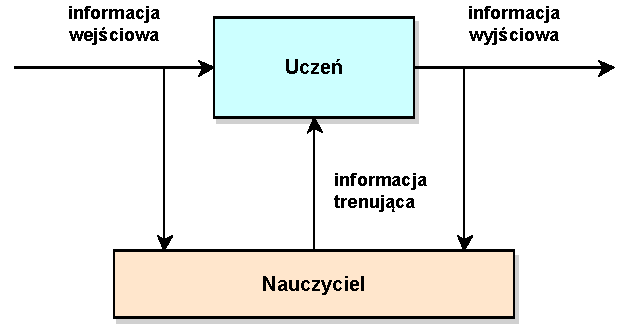
\includegraphics{graphics/01_podstawy_teoretyczne/supervised-learning.pdf}
	\caption{Uczenie maszynowe z nauczycielem \cite{CICHOSZ00}}
	\label{fig:supervised-learning}
\end{figure}

Uczeń otrzymuje od nauczyciela informację o tym jakiego komunikatu wyjściowego oczekuje w odpowiedzi na przykładowe informacje wejściowe. Mogą być one dostarczone np. w formie par składających się z wektorów danych oraz poprawnej odpowiedzi: $(x_{i}, y_{i})$. Na podstawie przykładów, system ma wyuczyć się przyporządkowywania danych do odpowiednich odpowiedzi. Innymi słowy, ma nauczyć się takiej funkcji $f$, dla której $f(x_{i})=y_{i}$, dla każdego $i$. Przykładami w uczeniu maszynowym mogą być różne obiekty, takie jak przedmioty, osoby, obserwacje.

Każdy przykład określany jest przez skończony oraz niepusty zbiór atrybutów $A=\lbrace a_{i}, a_{2}, \cdots, a_{n}\rbrace$. Atrybuty ze względu na rodzaj dziedziny możemy podzielić na: 
\begin{compactitem}
	\item nominalne, tj. takie, których dziedziny są zbiorami nieuporządkowanymi -- dla dwóch wartości możliwe jest określenie jedynie czy są równe czy nierówne,
	\item porządkowe, dla których dziedziny są zbiorami uporządkowanymi, czyli możliwe jest określenie relacji porządku liniowego na zbiorze wartości,
	\item liczbowe, których dziedziny są zdefiniowane jako zbiór liczbowy.
\end{compactitem}

W zależności od rodzaju odpowiedzi możemy wyróżnić dwa typowe rodzaje problemów, które stara się rozwiązać uczenie nadzorowane. Jeśli system ma przyporządkować do wektora wejściowego pojedynczą kategorię pochodzącą ze skończonego i dyskretnego zbioru kategorii, wówczas określamy ten problem jako problem kategoryzacji. Natomiast w przypadku przyporządkowywania odpowiedzi składającej się z jednej lub więcej zmiennych ciągłych, mówimy o problemie regresji.\cite{BISHOP06} Proces działania maszyny realizującej uczenie nadzorowane możemy podzielić na dwa etapy: etap treningu lub też nauki oraz etap polegający na rozwiązywania przynależności nowych wektorów wejściowych, który często określa się jako testowanie lub walidację.

W uczeniu nienadzorowanym nie występuje rola nauczyciela, a co za tym idzie, do systemu nie trafiają informacje treningowe. Dostępne są jedynie wektory wejściowe i na podstawie ich obserwacji system ma nauczyć się odpowiednich odpowiedzi.\cite{CICHOSZ00} Podejście to nie polega zatem na przyporządkowaniu wektorów do ustalonych wcześniej kategorii, lecz na wyznaczeniu ukrytej struktury w danych, które są nieopisane.\cite{VALPOLA} Wykorzystywane jest m.in. do rozwiązywania problemu klasteryzacji (\emph{ang. clustering}), który polega na znajdowaniu grup podobnych obiektów wśród danych wejściowych. Ponadto uczenie nienadzorowane wykorzystywane jest to określania rozkładu danych w przestrzeni wejściowej, co nazywamy szacowaniem rozkładu (\emph{ang. density estimation}) lub do rzutowania danych z przestrzeni wielowymiarowej do trójwymiarowej w celu dokonania wizualizacji.\cite{BISHOP06}

Na rys. \ref{fig:unsupervised-learning} przedstawiono uproszczony schemat mechanizmu uczenia nienadzorowanego. Algorytm uczący dokonuje podziału zestawu danych na klastry, które następnie muszą zostać zinterpretowane przez człowieka. W zaprezentowanym przykładzie klastry zostały nazwane na podstawie analizy ich zawartości. W rzeczywistych problemach zadanie nadania etykiet wytworzonym klastrom może okazać się trudne i może wymagać dostrojenia parametrów algorytmu by identyfikacja klastrów była możliwa.

\begin{figure}[h]
	\centering
	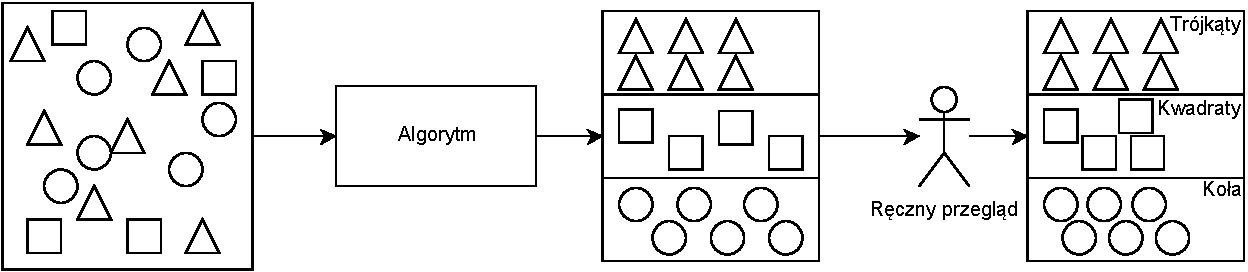
\includegraphics[scale=0.77]{graphics/01_podstawy_teoretyczne/unsupervised-learning.pdf}
	\caption{Uczenie maszynowe nienadzorowane \cite{CASEY}}
	\label{fig:unsupervised-learning}
\end{figure}

Dane wejściowe z etapu walidacji mogą się różnić od przykładowych danych służących do wytrenowania systemu. Umiejętność udzielania poprawnej odpowiedzi na komunikaty, które różnią się od przykładowych danych określamy jako generalizacja.\cite{BISHOP06}
%TODO napisac o tym w kontekscie pracy, co raczej sie nadaje a co raczej nie

Wśród dostępnych publikacji na temat kategoryzacji obrazów przeważają rozwiązania oparte na uczeniu nadzorowanym lub pól-nadzorowanym.\cite{MELE06}\cite{CHEN04}\cite{Vitaladevuni13}\cite{LUO11} Istnieje jednak kilka rozwiązań opartych na uczeniu nienadzorowanym, m.in. w  Dai D., Wu T., Zhu S-c., \emph{Discovering Scene Categories by Information Projection and Cluster Sampling}\cite{DAI10} gdzie zaprezentowano metodę kategoryzacji sceny opartą na uczeniu nienadzorowanym, lub Huang Y., Liu Q., Lv F., Gong Y., Dimitris N., \emph{Unsupervised Image Categorization by Hypergraph Partition}\cite{HUANG11}, gdzie klastrowanie obrazów sformowano jako problem podziału hipergrafu.

\section{Rozpoznawanie wzorców}

%TODO sprawdzic wzory

Celem rozpoznawania wzorców (\emph{ang. pattern recognition}) jest stworzenie symbolicznego opisu dla zawartości jedno lub wielowymiarowego sygnału cyfrowego takiego jak np. cyfrowy obraz graficzny, sygnał mowy, lub obraz z kamery, a następnie przyporządkowanie do niego klasy lub instancji klasy. Opis ten może być zrealizowany w różnej formie: funkcji, obiektów, ruchu, wyrazów lub struktur.

Wzorcem nazywamy zbiór cech, który tworzy ilościowy oraz jakościowy opis obiektu. Wzorce zapisujemy najczęściej jako wektory, ciągi lub drzewa. Wzór \ref{pattern_vector} przedstawia wektor cech, gdzie $x_{i}$ reprezentuje $i$-tą cechę, a $n$ oznacza ilość wszystkich cech powiązanych ze wzorcem.\cite{GONZALES01}
\begin{equation} 
\label{pattern_vector} 
\overrightarrow{x}=
\begin{bmatrix}x_1\\
x_2\\
\vdots\\
x_n  
\end{bmatrix}
\end{equation}

Zbiór wzorców charakteryzujący się podobnymi wektorami cech nazywamy klasą wzorców i oznaczamy jako $\omega_1, \omega_2, \cdots, \omega_{W}$, gdzie dolny indeks określa numer klasy, a $W$ określa ilość klas. Jako rozpoznanie wzorca $\omega$ określa się przyporządkowanie wzorcowi jego klasy: $\overrightarrow{x} \rightarrow \omega$. Przestrzeń wektorów cech $X$ zostaje przekształcona w przestrzeń klas wzorców $\Omega$.

W systemach analizy obrazów możemy oprócz rozpoznania zdefiniować również dwa inne pojęcia: identyfikację oraz weryfikację. Gdy nie dysponujemy opisami klas wzorców, a jedynie przechowujemy wzorce referencyjne, celem systemu jest porównanie aktualnego wzorca z bazą referencyjną. Jeśli na podstawie określonej odległości pomiędzy parami wzorców system jest w stanie dokonać wyboru dokładnie jednego wzorca referencyjnego, to określamy takie rozwiązanie jako identyfikację. Natomiast jeśli możemy wybrać przynajmniej jeden ze wzorców referencyjnych to określamy takie rozwiązanie jako weryfikację.

\section{Selekcja cech}

%TODO sprawdzic wzory

W przypadku dużych i skomplikowanych obiektów, takich jak obrazy, proces uczenia może okazać się bardzo skomplikowany i czasochłonny. Konieczne jest przeprowadzenie procesu selekcji cech obrazu (\emph{ang. feature selection}), który polega na znalezieniu podzbioru cech opisujących obiekt w najlepszy sposób i zapewniający najwyższą jakość modelu klasyfikacji. Celem selekcji cech jest redukcja wymiarów przestrzeni cech, zwiększenie szybkości działania algorytmu uczącego, zwiększenie dokładności klasyfikacji oraz osiągnięcie łatwiejszych do zrozumienia rezultatów uczenia.\cite{MOTODA98}

Wyselekcjonowane cechy powinny się charakteryzować następującymi właściwościami\cite{STRUMIL}:

\begin{compactitem}
	\item \emph{dyskryminacja} -- cechy powinny przyjmować jak najbardziej odmienne wartości dla obiektów z różnych klas,
	\item \emph{niezawodność} -- cechy powinny przyjmować podobne wartości dla wszystkich obiektów danej klasy,
	\item \emph{niezależność} -- cechy powinny nie być ze sobą skorelowane,
	\item \emph{małoliczność} -- im mniejsza liczba cech tym złożoność systemu jest mniejsza.
\end{compactitem}

Wzór \ref{correlation} przedstawia współczynnik korelacji cech $x$ i $y$. Jeśli współczynnik korelacji jest bliski $1$ lub $-1$ to cechy $x$ i $y$ są ze sobą silnie skorelowane i należy jedną z nich odrzucić.
\begin{equation} 
\label{correlation} 
\hat{\sigma}_{xy}= \frac{\frac{1}{P}\sum\limits_{i=1}^P(x_i-\mu_x)(y_i-\mu_y)}{ \hat{\sigma}_x\hat{\sigma}_y }
\end{equation} gdzie $P$ -- liczba klasyfikowanych obiektów, $\mu$ -- wartość średnia, $\sigma$ -- odchylenie standardowe zbioru cech.

Miarę separacji można określić jako:

\begin{equation}
	\hat{D}_{xjk} = \frac{|\mu_xj - \mu_xk|}{\sqrt{\hat{\sigma}^2_xj \hat{\sigma}^2_xk}}
\end{equation}

Duża wartość tej miary świadczy o dobrej separacji pomiędzy klasami $j$ i $k$.

Badanie jakości klasyfikacji dla wszystkich możliwych kombinacji podzbioru cech dla dużej liczby $N$ wszystkich cech jest bardzo kosztowne, dlatego w praktyce zbiór cech często dobierany jest intuicyjnie.\cite{STRUMIL}

%TODO Opis mRMR, CFS, http://en.wikipedia.org/wiki/Feature_selection

Po poprawnej selekcji cech, możliwe powinno się stać stworzenie takiego modelu, w którym cechy nie dające informacji potrzebnej do klasyfikacji lub takie, które są nadmiarowe lub pogarszają jakość klasyfikacji zostały wyeliminowane. Dążymy przy tym do osiągnięcia najmniejszego możliwego wektora cech. Opierając się na mniejszym, mniej wymiarowym wektorze cech, potrzeba mniej przykładów do osiągnięcia dobrych wyników klasyfikacji.

\section{Ekstrakcja cech}

Obrazy w formie map bitowych reprezentowane są w pamięci komputera w postaci macierzy pikseli. Ilość danych jest dla klasyfikacji zbyt duża i zawiera wiele niepotrzebnych informacji. Dlatego przed przystąpieniem do procesu klasyfikacji należy wydobyć z obrazu pewne cechy. Proces przetwarzania obrazu w celu wydobycia cech określa się jako ekstrakcję cech (\emph{ang. feature extraction}).

Można wyróżnić wiele cech używanych w procesach przetwarzania obrazów, np. rozkład kolorów w formie histogramu, obecność niektórych elementów lub kształtów, liczba występowania podobnych obiektów, wielkość kształtów, morfologia, tekstura. Przed ekstrakcją cech często warto przeprowadzić przetwarzanie wstępne (\emph{ang. preprocessing}) celem uzyskania obrazów o lepszych parametrach do ekstrakcji.

\section{Przegląd algorytmów do ekstrakcji cech}

Wśród popularnych metod ekstrakcji cech, stosowanych do rozwiązania problemu klasyfikacji i kategoryzacji obrazów należy wymienić: SIFT (\emph{ang. Scale-invariant Feature Transform})\cite{SIFT99}, SURF (\emph{ang. Speeded Up Robust Features}), GIST\cite{GIST09}, LBP (\emph{ang. Local Binary Patterns}), HOG (\emph{ang. Histograms of Oriented Gradients}). Poszczególne algorytmy zostały opisane poniżej.

\subsection{SIFT -- Scale-invariant Feature Transform}

Algorytm SIFT służy do wykrywania oraz opisu lokalnych cech obrazu, został opublikowany przez Dawida Lowe w 1999 roku.\cite{SIFT99} Punkty charakterystyczne wykrywane przez SIFT są niezmiennicze względem położenia, rotacji, skali, zmiany oświetlenia oraz są odporne na zakłócenia. Zastosowanie algorytmu SIFT do rozpoznawania obiektów pozwala na detekcję częściowo zasłoniętych obiektów. Jest to jeden z najpopularniejszych algorytmów do ekstrakcji punktów charakterystycznych.

Działanie algorytmu rozpoczyna się od wyszukiwania potencjalnych punktów poprzez przetworzenie obrazu filtrem Gaussa w różnych skalach. Stanowi to implementację tzw. przestrzeni skal (\emph{ang. skale space}). Przestrzeń skal definiujemy jako funkcję $L(x, y, \sigma)$. Wzór \ref{sift_scale_space} przedstawia reprezentację przestrzeni skal po przetworzeniu obrazu $I(x, y)$:
\begin{equation} 
\label{sift_scale_space} 
L(x, y, \sigma) = G(x, y, \sigma) \ast I(x, y)
\end{equation} gdzie $G(x, y, \sigma)$ -- Gaussian, $I(x, y)$ -- obraz wejściowy, $\ast$ -- operator splotu.
\begin{equation} 
\label{sift_gaussian} 
G(x, y, \sigma) = \frac{1}{2\pi\sigma^2}e^{-(x^2+y^2)/2\sigma^2}
\end{equation} 

W celu optymalnego wykrywania stabilnych punktów charakterystycznych, zaproponowano użycie ekstremum przestrzeni skal dla funkcji DOG (\emph{ang. difference-of-Gaussian}) w splocie z obrazem, oznaczone jako $D(x, y, \sigma)$.

Różnicowy filtr Gaussa (DOG) dla dwóch skal rozdzielonych współczynnikiem $k$ można zapisać jako:
\begin{equation} 
\label{sift_dog} 
G(x, y, k\sigma) - G(x, y, \sigma) 
\end{equation} 

Stąd wynik spotu obrazu z filtrem DOG można zapisać jako:
\begin{equation} 
\label{sift_splot} 
	\begin{gathered}
		D(x, y, \sigma) = [G(x, y, k\sigma) - G(x, y, \sigma)] \ast I(x, y) \\
		D(x, y, \sigma) = L(x, y, k\sigma) - L(x, y, \sigma)
	\end{gathered}
\end{equation}

Na rys. \ref{fig:sift-gaussian-to-dog} przedstawiono efektywny sposób konstruowania $D(x, y, \sigma)$. Obraz wejściowy fitrowany jest iteracyjnie filtrem Gaussa w różnych skalach rozdzielonych stałym współczynnikiem $k$ w celu wytworzenia obrazów oddalonych od siebie o współczynnik $k$ w przestrzeni skali (lewa kolumna).

Przestrzeń skal jest dzielona na oktawy, które reprezentują serię map odpowiedzi filtra uzyskane przez obliczenie splotu obrazu z filtrem. Zwiększenie skali o oktawę oznacza zwiększenie wygładzania o 2. Każda oktawa jest dzielona na liczbę całkowitą $s$, określającą liczbę interwałów, więc $k=2^{1/s}$. Należy zatem wyprodukować $s+3$ obrazów dla każdej oktawy, tak aby końcowe ekstremum pokrywało całą oktawę. Obrazy z sąsiednich skal są następnie odejmowane od siebie w celu otrzymania różnicy gaussianów DOG. Procedurę powtarza się próbkując obraz gaussowski poprzez usunięcie co drugiego wiersza i kolumny obrazu.\cite{LOWE04}

\begin{figure}[h]
	\centering
	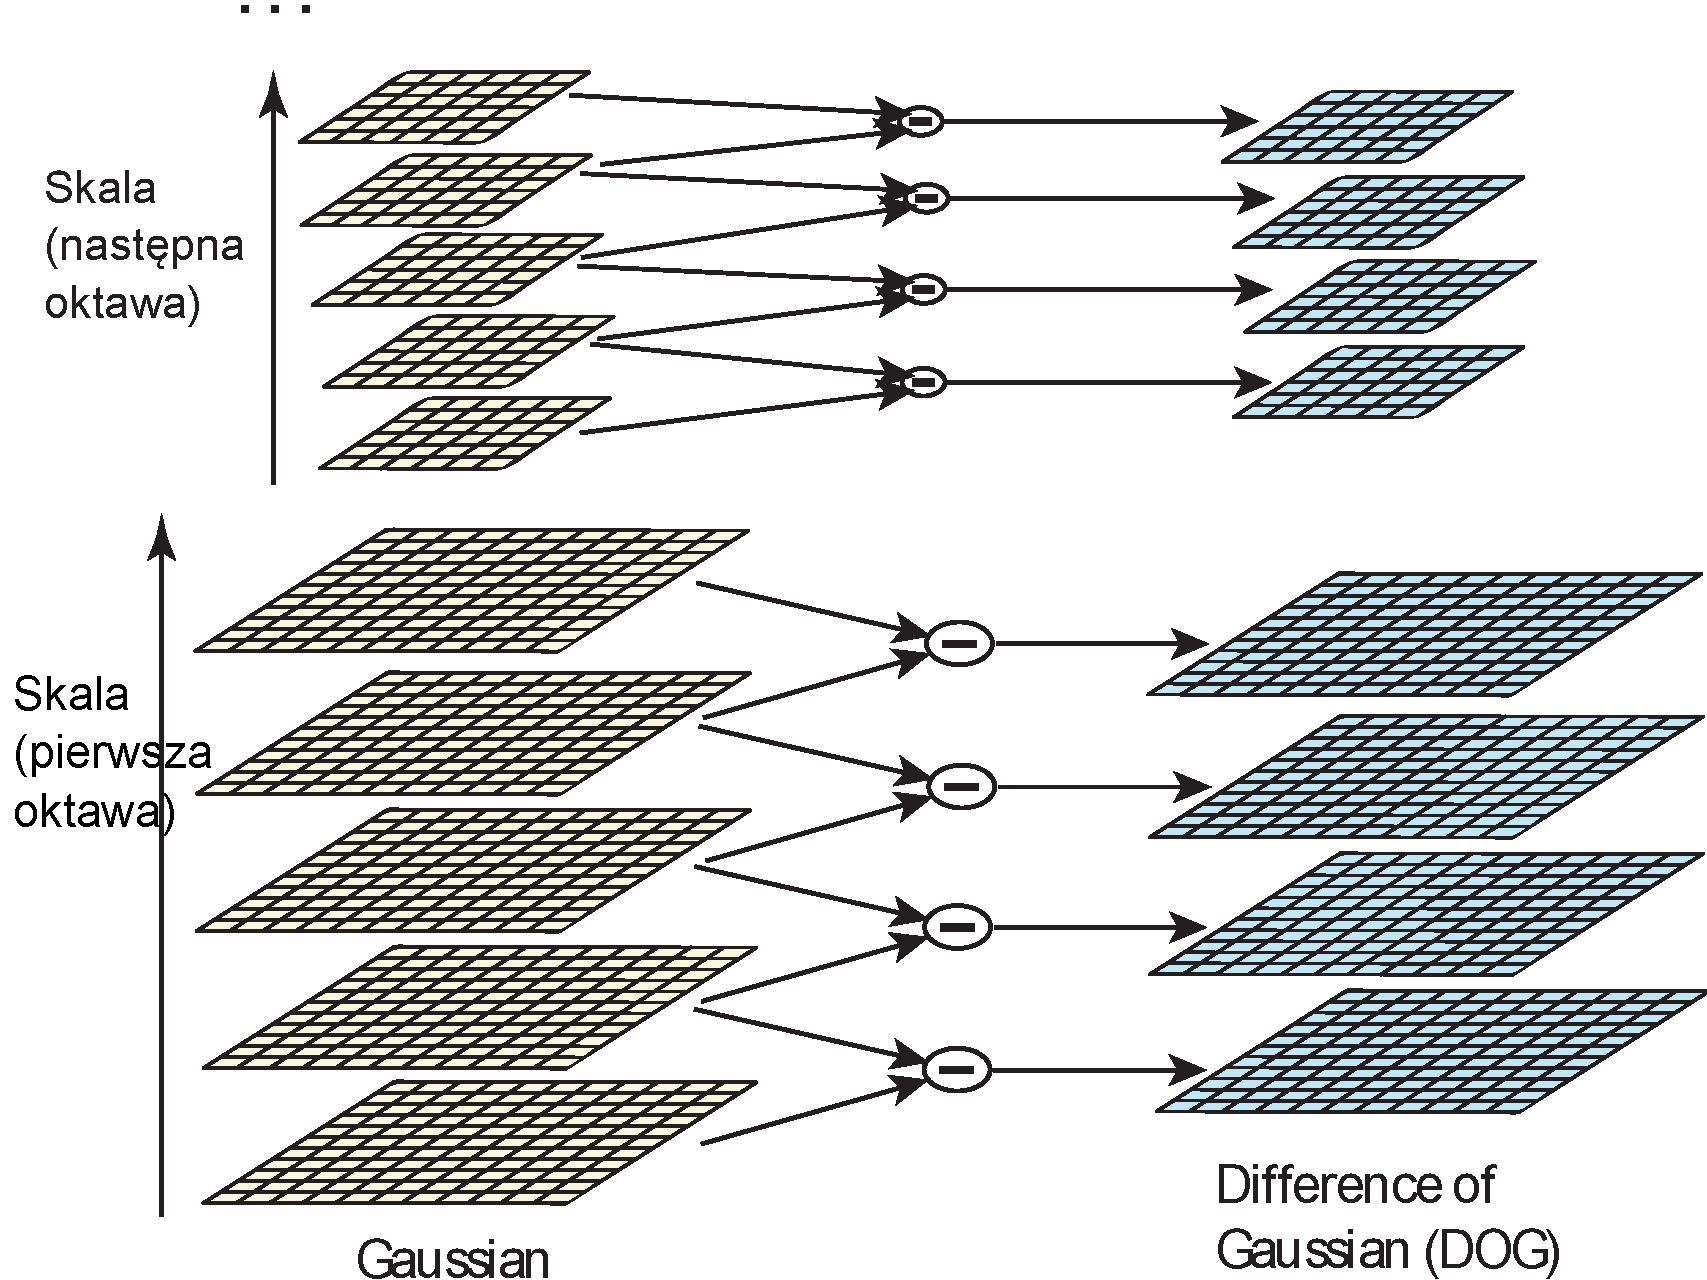
\includegraphics[scale=0.4]{graphics/01_podstawy_teoretyczne/sift-gaussian-to-dog.pdf}
	\caption{Proces tworzenia różnicy Gaussianów w algorytmie SIFT \cite{LOWE04}}
	\label{fig:sift-gaussian-to-dog}
\end{figure}

W celu wykrycia lokalnych ekstremów, punkty są porównywane z sąsiadami w otoczeniu 3x3x3, tj. po dziewięć sąsiadów w skalach poniżej i powyżej oraz z ośmioma sąsiadami w aktualnej skali. Punkt jest przyjmowany jako kandydat na punkt charakterystyczny tylko wówczas gdy ma wartość mniejszą lub większą od wszystkich 26 punktów sąsiednich.\cite{LOWE04} Rys. \ref{fig:sift-gaussian-min-max} przedstawia porównanie punktu, oznaczonego na schemacie za pomocą "X", z punktami sąsiednimi.

\begin{figure}[h]
	\centering
	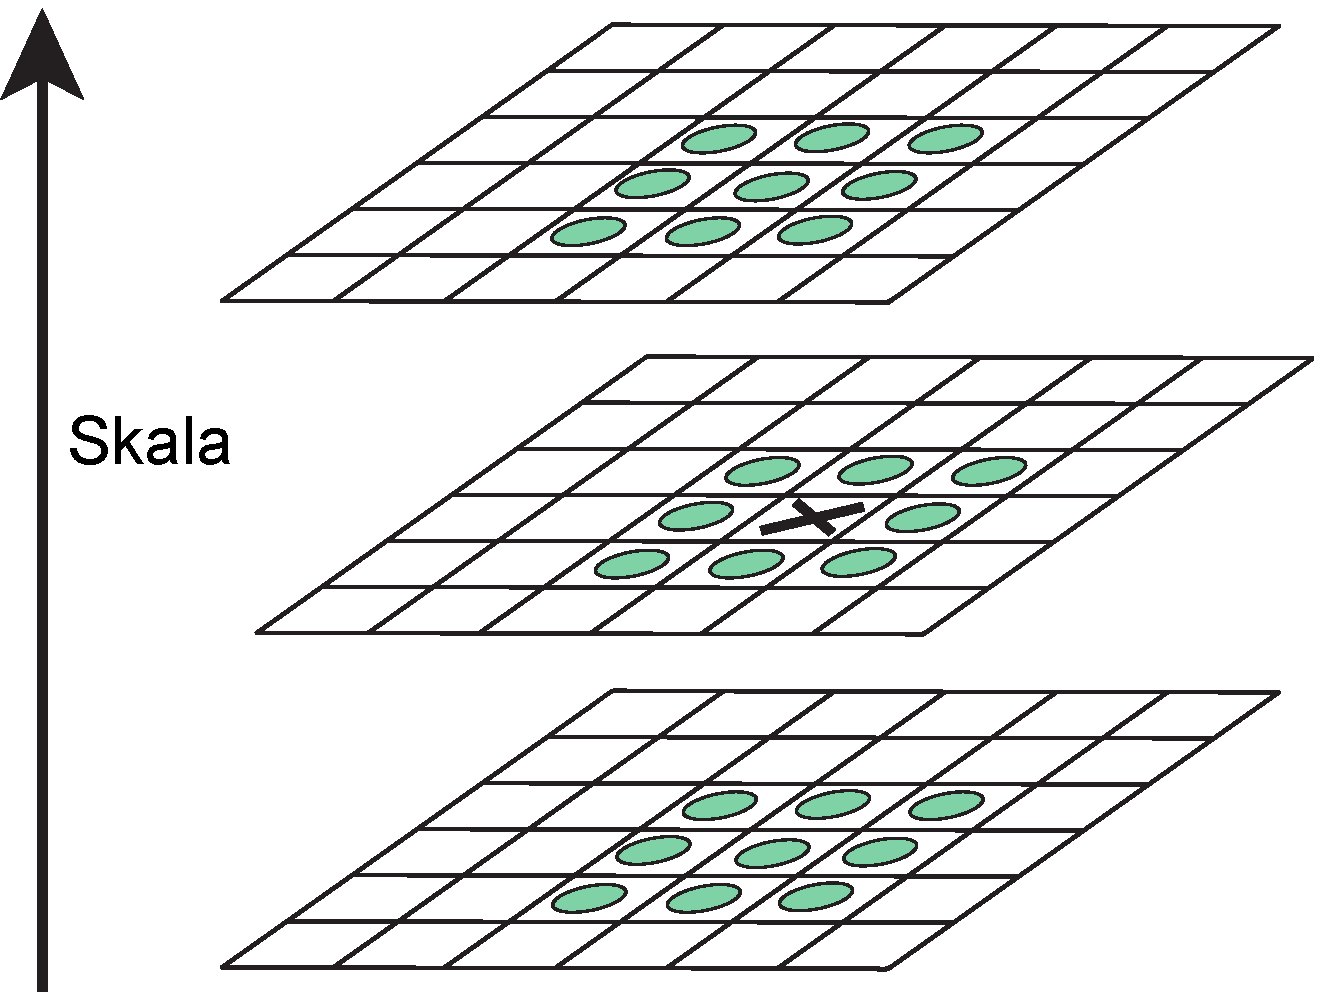
\includegraphics[scale=0.4]{graphics/01_podstawy_teoretyczne/sift-gaussian-min-max.pdf}
	\caption{Porównanie punktu z sąsiadami \cite{LOWE04}}
	\label{fig:sift-gaussian-min-max}
\end{figure}

Po znalezieniu kandydatów następuje lokalizacja punktów charakterystycznych. Proces ten odbywa się poprzez interpolację ekstremów dla kandydatów wyznaczonych w poprzednim punkcie za pomocą funkcji kwadratowej 3D:
\begin{equation} 
\label{sift_3d} 
D(x) = D + \frac{\partial D^T}{\partial x} x + \frac{1}{2}x^T \frac{\partial^2 D}{\partial x^2} x
\end{equation}

Dokładne położenie ekstremum wyznacza się na podstawie pochodnej funkcji $D(x)$:
\begin{equation} 
\label{sift_pochodna_D} 
\hat{x} = -\frac{\partial^2 D^-1}{\partial x^2}\frac{\partial D}{\partial x}
\end{equation}

Wartość funkcji w punkcie ekstremum służy do odrzucania niestabilnych punktów ze względu na mały kontrast. Wzór można uzyskać poprzez podstawienie wzoru \ref{sift_pochodna_D} do \ref{sift_3d}:
\begin{equation} 
\label{sift_Dx} 
D(\hat{x}) = D + \frac{1}{2} \frac{\partial D^T}{\partial x} \hat{x}
\end{equation}

Funkcja DOG będzie mieć dużą odpowiedź wzdłuż krawędzi. Za Harris i Stephens (1988), punkty ekstremum będące odpowiedzią wzdłuż krawędzi na obrazie są odrzucane na podstawie warunku \ref{sift_warunek}:
\begin{equation} 
\label{sift_warunek} 
\frac{\Tr(\boldsymbol{H})^2}{\Det(\boldsymbol{H})} < \frac{(r+1)^2}{r}
\end{equation} gdzie Hessian ma postać macierzy:
\begin{equation} 
\label{sift_hessian} 
\boldsymbol{H} = 
	\begin{bmatrix}
		D_{xx} & D_{xy} \\
		D_{xy} & D_{yy}
	\end{bmatrix}
\end{equation} oraz $r$ jest stosunkiem największej wartości własnej macierzy do najmniejszej.

Orientacja punktów wyznaczana jest na podstawie jednego z obrazów gaussowskich, którego skala odpowiada skali danego punktu charakterystycznego. Dla każdej próbki obrazu $L(x, y)$ obliczane są moduł gradientu $m(x, y)$ oraz orientacja $\theta(x, y)$:
\begin{equation} 
\label{sift_gradient_magnitude} 
m(x, y) = \sqrt{(L(x + 1, y) - L(x - 1, y))^2 + (L(x, y + 1) - L(x, y - 1))^2}
\end{equation}

\begin{equation} 
\label{sift_orientation} 
\theta(x, y) = \tan^{-1}((L(x, y + 1) - L(x, y - 1))/L(x + 1, y) - L(x - 1, y)))
\end{equation}

Na podstawie orientacji punktów, w otoczeniu punktu charakterystycznego budowany jest histogram orientacji. Maksimum w histogramie i lokalne maksima o wartościach powyżej 80\% największego maksimum lokalnego określają orientację punktu charakterystycznego. Przyjmuje się, że histogram posiada 36 pól, a dokładne położenie maksimum interpoluje się za pomocą paraboli korzystając z wartości sąsiednich histogramu.

Dzięki temu, że wszystkie cechy punktów charakterystyczne są mierzone w odniesieniu do tak wyznaczonej orientacji, opis jest niezmienniczy względem rotacji.

SIFT do opisu cech wykorzystuje moduł gradientu oraz orientację z otoczenia 16x16 dla danego punktu charakterystycznego. Obszar ten jest dzielony na podregiony 4x4, w których również wyznacza się wypadkowe histogramy orientacji. W każdym obszarze dla 8 orientacji wyznacza się wypadkowy moduł gradientu na podstawie modułów poszczególnych punktów. Na rys. \ref{fig:sift-descriptor} został przedstawiony przykład wyznaczenia wypadkowego gradientu dla otoczenia 8x8 i podregionów 2x2.

\begin{figure}[h]
	\centering
	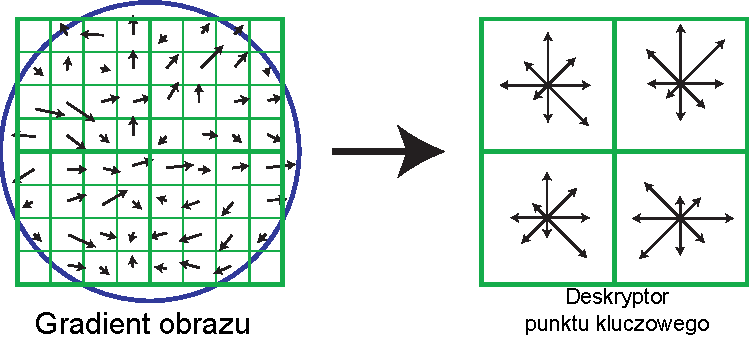
\includegraphics[scale=1]{graphics/01_podstawy_teoretyczne/sift-descriptor.pdf}
	\caption{Wyznaczenie deskryptora SIFT o rozmiarze 2x2 z otoczenia 8x8 \cite{LOWE04}}
	\label{fig:sift-descriptor}
\end{figure}

W celu rozpoznania obiektów za pomocą algorytmu SIFT należy najpierw wyznaczyć punkty charakterystyczne i odpowiadające im wektory cech lokalnych, a następnie dopasować punkty charakterystyczne z obrazu wejściowego do punktów w bazie wzorców. Do identyfikacji grup dopasowanych punktów, które określają ten sam obiekt wykorzystuje się transformatę Hougha. Weryfikacji cech dokonuje się z wykorzystaniem metody najmniejszych kwadratów. W trakcie obliczeń wyznaczane są parametry związane z transformacją pomiędzy układem związanym z wzorcem a układem związanym z obiektem na badanym obrazie.

\subsection{SURF -- Speeded Up Robust Features}

SURF jest kolejnym algorytmem do wykrywania lokalnych cech obrazu. Został zaproponowany w 2006 roku przez Herberta Bay'a i jest częściowo wzorowany na algorytmie SIFT.\cite{BAY08} Algorytm jest odporny zarówno na zmiany skali jak i zmiany rotacji. Wykorzystywany jest do rozpoznawania obiektów jak i rekonstrukcji scen 3D. Typowa implementacja jest nawet kilka razy szybsza od algorytmu SIFT.\cite{SCHWEIGER09}

W celu optymalizacji działania filtrów splotowych zastosowano obrazy całkowe (\emph{ang. integral images}). Pozycja w obrazie całkowym $I_{\Sigma}(\boldsymbol{x})$ w punkcie $\boldsymbol{x}=(x, y)^T$ reprezentuje sumę intensywności wszystkich pikseli wejściowego obrazu $I$ wewnątrz prostokąta pomiędzy początkiem układu współrzędnych a $x$.
\begin{equation} 
\label{surf_integral_image} 
I_{\Sigma}(\boldsymbol{x}) = \sum\limits_{i=0}^{i \leq x} \sum\limits_{j=0}^{j \leq y} I(i,j)
\end{equation}

Zastosowanie obrazu całkowego (\emph{ang. integral image}) pozwala ograniczyć ilość operacji dla sumowania intensywności oraz uniezależnić czas obliczeń od wielkości filtra.\cite{BAY08}

Ze względów wydajnościowych, wyszukiwanie punktów charakterystycznych oparte zostało na Hessianie. Dla punktu $\boldsymbol{x}=(x, y)$ na obrazie $I$, Hessian $H(\boldsymbol{x}, \sigma)$ w punkcie $\boldsymbol{x}$ i w skali $\sigma$ został zdefiniowany we wzorze \ref{surf_hessian}.
\begin{equation} 
\label{surf_hessian} 
H(\boldsymbol{x}, \sigma) = 
	\begin{bmatrix}
		L_{xx}(\boldsymbol{x}, \sigma) & L_{xy}(\boldsymbol{x}, \sigma) \\
		L_{xy}(\boldsymbol{x}, \sigma) & L_{yy}(\boldsymbol{x}, \sigma)
	\end{bmatrix}
\end{equation} gdzie $L_{xx}(\boldsymbol{x}, \sigma)$ -- splot drugiej pochodnej Gaussiana $\frac{\partial^2}{\partial x^2} g(\sigma)$ z obrazem $I$ w punkcie $\boldsymbol{x}$.

O ile zastosowanie Gaussianów jest optymalne\cite{LINDENBERG90}, to jednak ma obniżoną powtarzalność przy rotacji dla nieparzystych wielokrotności $\frac{\pi}{2}$. Korzystając z tych obserwacji, w algorytmie SURF zaproponowano przybliżenie oparte na filtrze pudełkowym, w celu zwiększenia wydajności. Na rys. \ref{fig:surf-box-filters} zostało przedstawione porównanie laplacianów $L_{yy}$ (a), oraz $L_{xy}$ (b), oraz odpowiadające im przybliżenia: $D_{yy}$ (c) oraz $D_{xy}$ (d).

\begin{figure}[h]
	\centering
	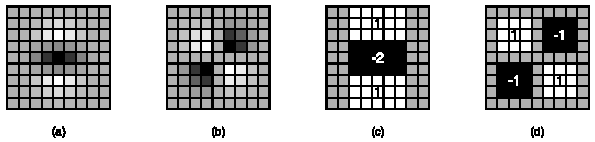
\includegraphics[scale=1.7]{graphics/01_podstawy_teoretyczne/surf-box-filters.pdf}
	\caption{Porównanie filtrów Gaussa z filtrami pudełkowymi 9x9 (skala $\sigma = 1.2$) \cite{BAY08}}
	\label{fig:surf-box-filters}
\end{figure}

Wyznacznik przybliżonej wartości Hessiana $H$ można zapisać jako:
\begin{equation} 
\label{surf_hessian_det}
\det(H_{approx}) = D_{xx} D_{yy} - (w D_{xy})^2
\end{equation}

Waga odpowiedzi filtra $w$ służy do zrównoważenia wyrażenia, dla zachowania energii pomiędzy maską Gaussa a przybliżoną maską Gaussa.
\begin{equation} 
\label{surf_hessian_approx_w}
w = \frac{|L_{xy}(1.2)|_F |D_{yy}(9)|_F}{|L_{yy}(1.2)|_F |D_{xy}(9)|_F} = 0.912... \simeq 0.9
\end{equation} gdzie $|A|_F$ -- norma Froberiusa (wzór \ref{surf_froberius}).
\begin{equation} 
\label{surf_froberius}
|A|_F = \sqrt{\sum\limits_{i=1}^m \sum\limits_{j=1}^n |a_{ij}|^2}
\end{equation}

Ze względu na teoretyczną dokładność, wagi $w$ powinny zmieniać się wraz ze skalą, jednakże w praktyce nie ma to dużego wpływu na precyzję wyników, w związku z tym przyjmuje się stałe $w = 0.9$. Przybliżone wyznaczniki Hessianów reprezentują odpowiedź obszarów spójnych ({ang. blob}) w punkcie $x$. Odpowiedzi filtra są normalizowane tak aby zachować stałą normę Frobeniusa dla każdego rozmiaru filtra.

W przypadku algorytmu SIFT, w celu uzyskania odpowiedniej skali, filtrowaliśmy obraz iteracyjnie tym samym filtrem. W algorytmie SURF, dzięki zastosowaniu obrazów całkowych, można zastosować bezpośrednio na obrazie wejściowym filtr pudełkowy o odpowiednim rozmiarze. Dzięki temu obrazy o różnych skalach można uzyskać nawet równolegle. 

Konstrukcja przestrzeni skal rozpoczyna się od filtra 9x9, który oblicza odpowiedź obszaru spójnego obrazu dla najmniejszej skali. Każda oktawa jest dzielona na stałą liczbę poziomów skalowania. Ze względu na dyskretny charakter obrazów całkowych, minimalna różnica skali pomiędzy dwoma kolejnymi poziomami zależy od długości $l_0$, która określa rozmiar obszaru o jednakowych wartościach (1, -1, -2) na filtrze. W przypadku filtra 9x9 wartość ta wynosi 3.

Dla dwóch kolejnych poziomów wartość tą należy zwiększyć przynajmniej o 2 piksele oraz zapewnić wystąpienie środkowego piksela, w rezultacie wielkość filtra zwiększa się o 6 pikseli pomiędzy poziomami. Porównanie filtrów 9x9 z filtrami 15x15 przedstawiono na rys. \ref{fig:surf-9-to-15}.

\begin{figure}[h]
	\centering
	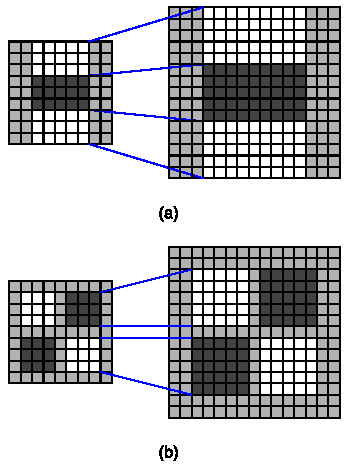
\includegraphics[scale=1.5]{graphics/01_podstawy_teoretyczne/surf-9-to-15.pdf}
	\caption{Porównanie filtrów pudełkowych 9x9 z filtrami 15x15: (a) $D_{yy}$, (b) $D_{xy}$ ($\sigma = 1.2$) \cite{BAY08}}
	\label{fig:surf-9-to-15}
\end{figure}

Dla kolejnych oktaw różnica pomiędzy poziomami jest zwiększana dwukrotnie, tj. wynosi 12 dla drugiej oktawy, 24 dla trzeciej, 48 dla czwartej itd. Algorytm może analizować wiele oktaw, jednak z każdą kolejną, ilość wykrytych punktów charakterystycznych maleje. Na rys. \ref{fig:surf-octaves} przedstawiono wielkości filtrów dla kilku kolejnych oktaw. Filtry w kolejnych oktawach nachodzą na siebie tak aby pokryć wszystkie możliwe skale.

\begin{figure}[h]
	\centering
	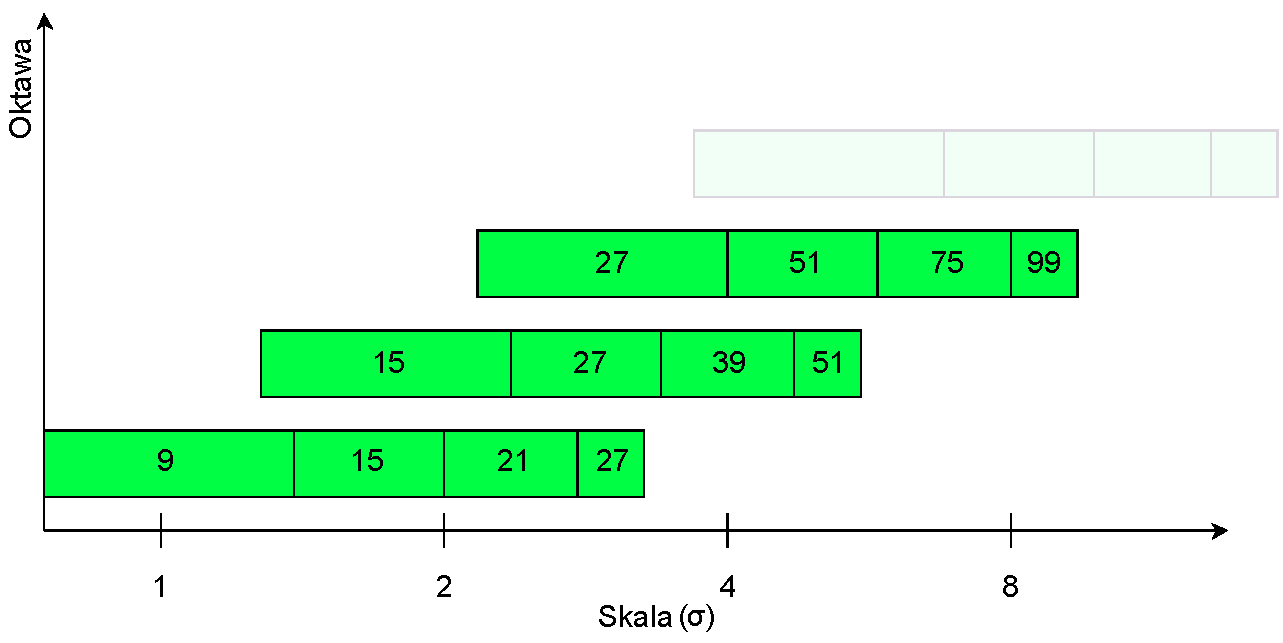
\includegraphics[scale=0.7]{graphics/01_podstawy_teoretyczne/surf-octaves.pdf}
	\caption{Wielkości filtrów pudełkowych dla kilku kolejnych oktaw \cite{BAY08}}
	\label{fig:surf-octaves}
\end{figure}

W celu zlokalizowania punktów charakterystycznych wykorzystywana jest szybka metoda usuwania niemaksymalnych pikseli (\emph{ang. Non-Maximum Suppresion}) zaproponowana przez Neubecka i Van Goola\cite{NEUBECK06}. Podobnie jak w algorytmie SIFT, punkty te są wyszukiwane w otoczeniu 3x3x3.

Deskryptor SURF opisuje rozkład intensywności dla punktów charakterystycznych. W celu czasu obliczeń zastosowano odpowiedzi falek Haara w kierunkach $x$ i $y$ dla otoczenia punktów charakterystycznych o promieniu $6s$, gdzie $s$ jest skalą na której został wykryty punkt charakterystyczny. Wielkości filtrów Haara są zależne od skali stąd ich wielkość została określona na $4s$. Na rys. \ref{fig:surf-haar-wavelet} przedstawiono filtr Haara dla kierunku $x$ (a) oraz $y$ (b).

\begin{figure}[h]
	\centering
	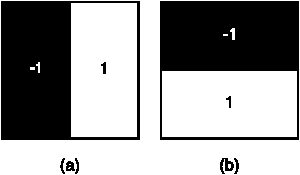
\includegraphics[scale=1.5]{graphics/01_podstawy_teoretyczne/surf-haar-wavelet.pdf}
	\caption{Filtry falkowe Haara do obliczenia odpowiedzi w kierunku $x$ (a) oraz $y$ (b) \cite{BAY08}}
	\label{fig:surf-haar-wavelet}
\end{figure}

Odpowiedzi filtra Haara sa następnie filtrowane za pomocą filtra Gaussa z $\sigma = 2s$ w celu wyeliminowania odkształceń. Na podstawie otrzymanych punktów, obliczane są sumy odpowiedzi w oknach o wielkości $\frac{\pi}{2}$, a następnie najdłuższy wektor z wszystkich okien definiuje się jako orientację punktu charakterystycznego.

Ekstrakcja rozpoczyna się od stworzenia kwadratowego obszaru wokół punktu charakterystycznego o wielkości $20s$. Obszar jest dzielony na podregiony 4x4, a następnie dla każdego podregionu, obliczane są odpowiedzi filtra Haara dla równo rozmieszczonych punktów w 5 rzędach i 5 kolumnach. Odpowiedzi  w kierunku $x$ oznaczane są jako $d_x$, natomiast odpowiedzi w kierunku $y$ oznaczane są jako $d_y$. Odpowiedzi $dx$ i $dy$ są następnie sumowane dla każdego podregionu i zostają umieszczone w wektorze cech. W celu określenia polaryzacji zmian intensywności, ekstraktuje się również sumę wartości bezwzględnych $|d_x|$ oraz $|d_y|$. W rezultacie każdy podregion otrzymuje czterowymiarowy wektor $\boldsymbol{v}$ określający strukturę intensywności.
\begin{equation} 
\label{surf_v_vector} 
\boldsymbol{v} = (\sum{d_x}, \sum{d_y}, \sum{|d_x|}, \sum{|d_y|})
\end{equation}

W rezultacie otrzymujemy wektor o długości równej 64. Odpowiedzi filtra Haara są niezmiennicze względem oświetlenia, natomiast niezmienniczość względem kontrastu jest otrzymywana poprzez wyliczenie wektora jednostkowego dla deskryptora.

\subsection{Modele GIST}

Studia nad percepcją pokazały, że obserwator jest w stanie jednym spojrzeniem rozpoznać scenę z realnego świata. W czasie tego szybkiego procesu, w układzie wzrokowym człowieka (rys. \ref{fig:gist-vision-system}) tworzona jest przestrzenna reprezentacja świata zewnętrznego, która jest na tyle bogata, że pozwala zrozumieć sens sceny, rozpoznać kilka obiektów oraz zwrócić uwagę na istotne szczegóły. Ta reprezentacja, którą można odnieść zarówno do funkcji niskopoziomowych, takich jak kolor lub częstotliwość, jak i informacji wysokiego poziomu, takich jak obiekty lub aktywacja wiedzy semantycznej określana jest jako gist (ang. istota, sedno).

\begin{figure}[h]
	\centering
	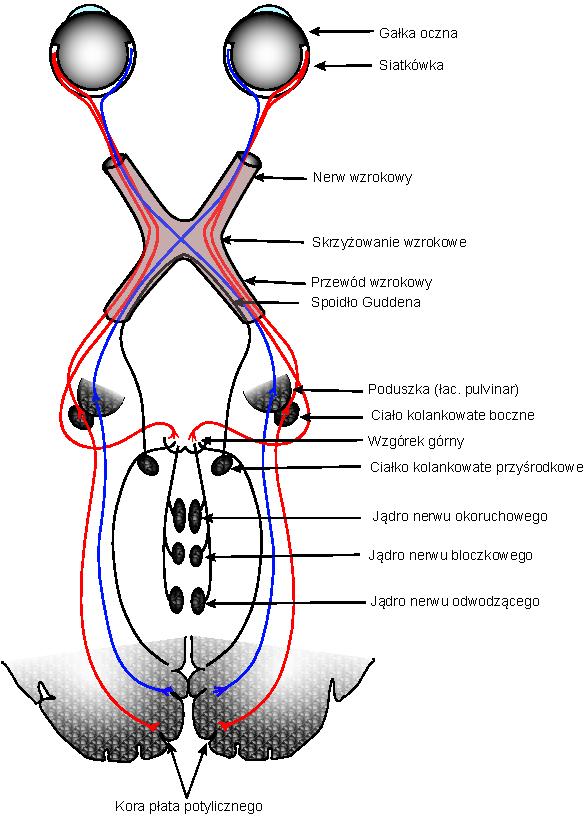
\includegraphics[scale=1.0]{graphics/01_podstawy_teoretyczne/gist-vision-system.pdf}
	\caption{Schemat układu wzrokowego człowieka \cite{GRAY18}}
	\label{fig:gist-vision-system}
\end{figure}

W czasie nie większym niż 100~ms, człowiek jest w stanie rozpoznać podstawowe kategorie obrazu, takie jak określenie miejsca, tj. czy obraz przedstawia ulicę, wnętrze mieszkania, las lub inną lokalizację\cite{POTTER76}, jak również jest w stanie rozpoznać układ przestrzenny zdjęcia, nawet jeśli jest ono nieostre.\cite{SCHYNS94} Potrafi także zapamiętać kilka obiektów, ich kontekst oraz niskopoziomową charakterystykę obszarów, które są najlepiej zauważalne.\cite{OLIVA05}

Cecha GIST w założeniu jest niskopoziomową reprezentacją sceny, która nie wymaga żadnej formy segmentacji. Podejście to nie jest alternatywą dla lokalnych cech obrazu ale może stanowić dodatkową pomoc przy rozpoznawaniu obiektów na nieuporządkowanej scenie.\cite{OLIVA06}

%-- Oliva Torralba 2000
%=================================================================================
Nie istnieje jeden model GIST. Oliva i Torralba w 2000 roku zaproponowali model, w którym rozkład przestrzenny widma został opisany przy pomocy okienkowej transformaty Fouriera (WFT), a następnie otrzymany wektor cech został zredukowany poprzez zastosowanie analizy głównych składowych (\emph{ang. PCA -- Principal Component Analysis}).\cite{OLIVA00} Okienkowa transformata Fouriera została określona przy pomocy wzoru \ref{gist_wft}:
\begin{equation} 
\label{gist_wft} 
I(x, y, f_x, f_y) = \sum\limits_{x^\prime, y^\prime = 0}^{N-1} i(x^\prime, y^\prime)h_r(x^\prime - x, y^\prime - y)e^{-j2\pi(f_xx^\prime+f_yy^\prime)}
\end{equation} gdzie $h_r(x^\prime, y^\prime)$ -- okno czasowe Hamminga

Wyznaczenie cech dla pojedynczego obrazu jest dla metody Oliva i Torralba bardzo szybkie i wynosi poniżej 1ms.

%-- Renninger Malik 2004
%=================================================================================
Renninger i Malik w 2004 zaproponowali inne rozwiązanie oparte na filtrach Gabora oraz ekstrakcji tekstonów. W zaproponowanym modelu wykorzystano pierwszą i drugą pochodną Gaussiana. Filtr składa się z dwóch faz -- parzystej i nieparzystej, opisanych we wzorze \ref{gist_gabor}.
\begin{equation} 
\label{gist_gabor} 
	\begin{gathered}
		f_{odd}(x, y) = {G^\prime}_{\sigma_1}(y) G_{\sigma_2}(x) \\
		f_{even}(x, y) = {G^{\prime\prime}}_{\sigma_1}(y) G_{\sigma_2}(x) 
	\end{gathered}
\end{equation} gdzie $G_\sigma(x)$ -- Gaussian z odchyleniem standardowym $\sigma$

Współczynniki $\sigma_1$ i $\sigma_2$ są miarami wydłużenia filtra. Filtry są budowane w 3 skalach dla zachowania selektywności częstotliwości oraz w 6 orientacjach dla selektywności orientacji. W rezultacie powstaje 36 filtrów. Podczas analizy tekstury, obliczany jest splot obrazu z zespołem filtrów, co w rezultacie daje wektor odpowiedzi $I \ast f(x_0, y_0)$ charakteryzujący fragment obrazu wyśrodkowany w $(x_0, y_0)$. 

Podobne tekstury na analizowanych obrazach powtarzają się bardzo często. W celu określenia jakie cechy są najbardziej powszechne użyto klastrowania K-średnich i otrzymano wektor składający się z 100 prototypowych odpowiedzi, które nazywamy \emph{uniwersalnymi tekstonami}. Ze względu na konieczność wyliczenia tekstonów rozwiązanie to jest dużo wolniejsze i wyliczenie cech dla obrazu zajmuje ok. 7 sekund.\cite{VISWANATHAN08}

%-- Siegian Itti 2007
%=================================================================================
W 2007 roku Siegian i Itti zaproponowali model składający się z biologicznie wiarygodnych cech określających orientację, kolor oraz intensywność.\cite{SIAGIAN07} Metoda ta powstała na kanwie badań nad percepcją, które wykazały, że obserwator jest w stanie określić ogólne, semantyczne atrybuty zdjęcia na podstawie ekspozycji nie przekraczającej 100~ms. Natomiast odpowiedź na bardziej specyficzne pytania, takie jak czy na zdjęciu znajduje się zwierzę, obserwator jest w stanie określić w czasie 28~ms\cite{THORPE95}, nawet wówczas gdy jego uwaga jest skupiona na innym zadaniu. Gist obrazu może być określany w obszarach mózgu, które odpowiadają za \emph{miejsca}, rozumiane jako typy sceny z określonym układem przestrzennym.\cite{EPSTEIN00} Układ przestrzenny oraz kolor zostały zostały doświadczanie określone jako cechy obrazu wpływające na dostrzeganie gistu sceny.\cite{OLIVA-SCHYNS00}

Model Siegiana i Itti opiera się na na \emph{saliency model} zaproponowanym wcześniej przez Itti. W modelu tym, obraz wejściowy jest filtrowany do wielu niskopoziomowych kanałów cech, w wielu skalach przestrzennych. Kanały takie jak kolor, orientacja i intensywność mają wiele podkanałów, które z kolei wyróżniają 9 poziomów skali od stosunku 1:1 (poziom 0) do 1:256 (poziom 8), wygładzone iteracyjnie filtrem Gaussa 5x5.

Dla każdego podkanału $i$ wykonywane są operacje porównania wartości centralnego punktu z jego sąsiedztwem, pomiędzy mapami wyjściowymi dla filtrów $O_i(s)$ w różnych skalach $s$. Mapy cech określamy jako $M_i(c, s)$, gdzie $c \in \{2, 3, 4\}$ -- skala centralna, $s = c + d$, $d \in \{3, 4\}$ -- skala otaczająca. Różnica między skalami zapisywana jest jako $\ominus$ i jest realizowane przez interpolację do skali centralnej i wyliczenie różnicy bezwzględnej. Zastosowanie skal $s$ oraz $c$ umożliwia zachowanie niezmienniczości względem oświetlenia.

Dla kanałów koloru i intensywności mamy:
\begin{equation} 
\label{gist_siegian_color_intensity}
M_i(c, s) = |O_i(c) \ominus O_i(s)| = |O_i(c) - Interp_{s-c}(O_i(s))|
\end{equation}

Kanał orientacji tworzony jest za pomocą filtrów Gabbora na obrazie w skali szarości, w czterech różnych kątach $\theta_i \in \{0, 45, 90, 135^\circ\}$ oraz dla czterech różnych skalach przestrzennych $c \in \{0, 1, 2, 3\}$, co daje łącznie 16 podkanałów. Mapy cech dla orientacji $M_i(c)$ określamy jako:
\begin{equation} 
\label{gist_siegian_orientation}
M_i(c) = Gabor(\theta_i, c)
\end{equation}

Kanały koloru i intensywności łączone są w celu stworzenia trzech par przeciwstawnych kolorów (\emph{ang. opponent colors}) z teorii barw przeciwstawnych Ewalda Heringa opisanej w \emph{Outlines of a Theory of the Light Sense}.\cite{HERING64} Niemiecki fizjolog Ewald Hering opisał cztery podstawowe kolory: czerwony, zielony, niebieski i żółty, ponadto wyróżnił dodatkowy składnik określony jako intensywność. Poniżej przedstawiono wzory na wyliczenie reprezentacji poszczególnych kanałów:
\begin{equation} 
\label{gist_hering_R} 
R = \frac{r - (g + b)}{2}
\end{equation}
\begin{equation} 
\label{gist_hering_G} 
G = \frac{g - (r + b)}{2}
\end{equation}
\begin{equation} 
\label{gist_hering_B} 
B = \frac{b - (r + g)}{2}
\end{equation}
\begin{equation} 
\label{gist_hering_Y} 
Y = r + g - 2 (|r - g| + b)
\end{equation}
\begin{equation} 
\label{gist_hering_I} 
I = \frac{r + g + b}{3}
\end{equation}

$R, G, B$ -- kanały czerwony, zielony i niebieski według Heringa, $r, g, b$ -- kanały czerwony, zielony i niebieski ze zdjęcia.

Pary kolorów przeciwstawnych tworzą kanały: czerwony i zielony, niebieski i żółty, dodatkowo wyróżniona jest para kanałów: ciemny i jasny. Kolory przeciwstawne nigdy nie są postrzegane razem, tj. nie ma czerwonawej zieleni ani niebieskawej żółci. Kanały kolorów przeciwstawnych zostały przedstawione na rys. \ref{fig:gist-opponent-colors}.

\begin{figure}[h]
	\centering
	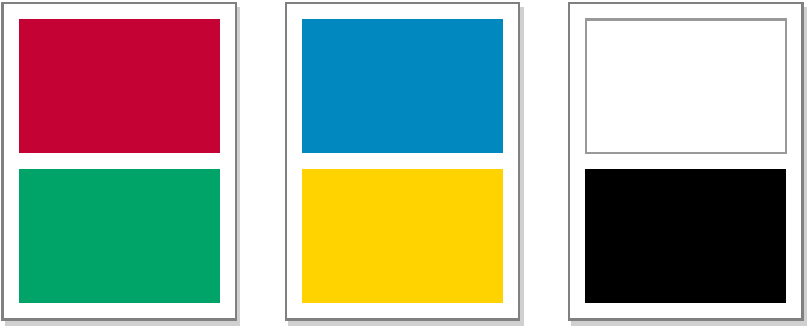
\includegraphics[scale=1.0]{graphics/01_podstawy_teoretyczne/gist-opponent-colors.pdf}
	\caption{ Pary kanałów kolorów przeciwstawnych (\emph{ang. opponent colors}) }
	\label{fig:gist-opponent-colors}
\end{figure}

Poszczególne pary można zapisać w postaci:
\begin{equation} 
\label{gist_siegian_RG} 
RG(c,s) = |(R(c) - G(c)) \ominus (R(s) - G(s))|
\end{equation}
\begin{equation} 
\label{gist_siegian_BY} 
BY(c, s) = |(B(c) - Y(c)) \ominus (B(s) - Y(s))|
\end{equation}
\begin{equation} 
\label{gist_siegian_I} 
I(c, s) = |I(c) \ominus I(s)|
\end{equation}

Każda z par jest używana do stworzenia sześciu kombinacji skal $s$ oraz $c$, co daje 18 kombinacji. Łącznie z kanałami orientacji otrzymujemy zatem 38 podkanałów.

Dla każdego podkanału wyliczany jest wektor GIST z odpowiadających map cech. Mapy dzielone są na podregiony 4x4, a następnie dla każdego podregionu wykonywane są operacje uśredniające. Wzór \ref{gist_siegian_G_kli} przedstawia obliczenia jakie należy wykonać dla każdej z 16 cech GIST na mapę dla koloru i intensywności. Analogiczne obliczenia stosuje się do wyliczenia $G_i^{k,l}(c)$ z map orientacji $M_i(c)$.
\begin{equation} 
\label{gist_siegian_G_kli} 
G_i^{k,l} = \frac{1}{16WH} \sum\limits_{u = \frac{kW}{4}}^{\frac{(k+1)W}{4} - 1} \sum\limits_{v = \frac{lH}{4}}^{\frac{(l+1)H}{4} - 1} [M_i(c, s)](u, v)
\end{equation} gdzie $k$ i $l$ -- indeksy poziomy i pionowy podregionu, $W$, $H$ -- szerokość i wysokość całego obrazu.

Łącznie map cech jest 34, co przy podziale na 16 regionów daje wektor o 544 wymiarach. W celu zmniejszenia wymiarowości stosuje się analizę głównych składowych -- PCA (\emph{ang. Principal Component Analysis}) oraz analizę składowych niezależnych -- ICA (\emph{ang. Independent Component Analysis}). Dzięki temu otrzymuje się wektor 80 wymiarowy.

Schemat procesu ekstrakcji cech GIST według Siegiana i Itti przedstawiono na rys. \ref{fig:gist-siagian}.

\begin{figure}[h]
	\centering
	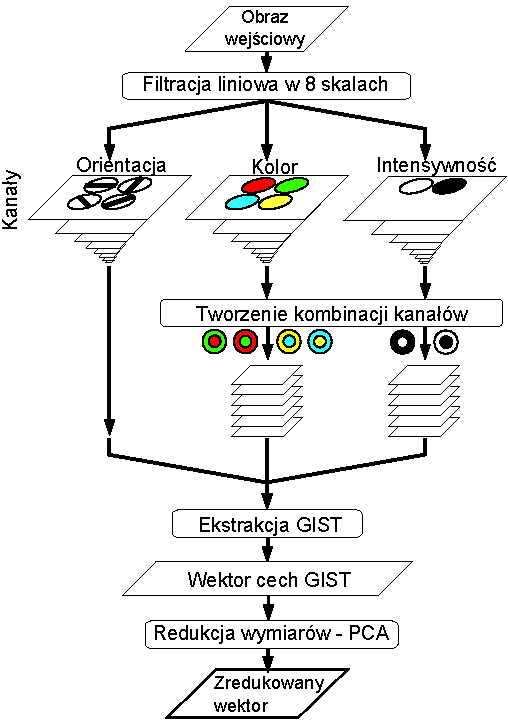
\includegraphics[scale=1.0]{graphics/01_podstawy_teoretyczne/gist-siagian.pdf}
	\caption{ Ekstrakcja cech GIST według Siegiana i Itti (2007) \cite{SIAGIAN07} }
	\label{fig:gist-siagian}
\end{figure}

Szybkość obliczeń rozwiązania zaproponowanego przez Siegiana i Itti jest podobna do rozwiązania Olivy i Torralbala z 2000 roku.

\subsection{LBP -- Local Binary Patterns}

Lokalny wzorzec binarny (\emph{ang. Local Binary Pattern, LBP}) jest bezparametrowym operatorem, który opisuje lokalną strukturę przestrzenną obrazu. Został zaproponowany po raz pierwszy przez Timo Ojala w \emph{A comparative study of texture measures with classification based on featured distributions}\cite{OJALA94} z 1994 roku, jako wysoce dyskryminujący dla klasyfikacji tekstur.

LBP dla pozycji $(x_c, y_c)$ zdefiniowany jest jako uporządkowany zestaw binarnych porównań intensywności pikseli pomiędzy centralnym pikselem a ośmioma pikselami otaczającymi w masce 3x3. Przykładowy LBP zaprezentowano na rys. \ref{fig:lbp-operator}.

\begin{figure}[h]
	\centering
	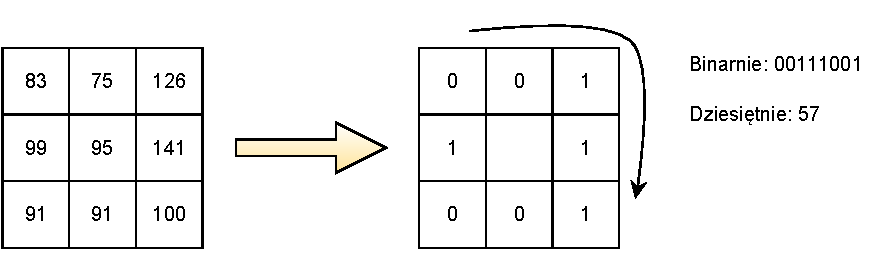
\includegraphics[scale=1.0]{graphics/01_podstawy_teoretyczne/lbp-operator.pdf}
	\caption{ Podstawowy operator LBP \cite{HEUSCH06} }
	\label{fig:lbp-operator}
\end{figure}

Wartość powstałego kodu LBP można wyrazić w postaci dziesiętnej jako:
\begin{equation} 
\label{lbp_lbp} 
LBP(x_c, y_c) = \sum\limits_{n = 0}^7 s(i_n - i_c) 2^n
\end{equation} gdzie $i_c$ -- wartość piksela $(x_c, y_c)$ w skali szarości, $i_n$ -- wartości 8 otaczających pikseli w skali szarości, natomiast funkcja $s$ zdefiniowana jest następująco:
\begin{equation} 
\label{lbp_s} 
s(x) = 
	\begin{cases}
		1 & \text{ jeżeli } x \geq 0 \\
		0 & \text{ jeżeli } x < 0
	\end{cases} 
\end{equation}

Każdy bit LBP jest w takim samym stopniu ważny, ale dwa dodatnie bity mogą mieć całkowicie inne znaczenie. Operator LBP nie zmienia się poprzez zastosowanie jakichkolwiek monotonicznych transformacji na skali szarości, ponieważ zachowują one porządek intensywności pikseli w lokalnym sąsiedztwie.

W 2002 roku, Ojala rozszerzył oryginalny operator LBP do okrągłego sąsiedztwa o różnych wielkościach promienia.\cite{OJALA02} Nową reprezentację określa się jako $LBP_{P, R}$:
\begin{equation} 
\label{lbp_lbp_pr} 
LBP_{P, R} = \sum\limits_{p=0}^{P-1} s(g_p - g_c) 2^P
\end{equation} gdzie $P$ -- ilość równo rozmieszczonych pikseli, $R$ -- promień, $g_c$ --  wartość centralnego piksela w skali szarości, $g_p (P = 0, \ldots, P-1)$ -- wartości pikseli z sąsiedztwa.

Na rys. \ref{fig:lbp-pr-operator} przedstawiono rozszerzony operator LBP dla sąsiedztwa $(8, 2)$, tj. $P = 8$, $R = 2$.

\begin{figure}[h]
	\centering
	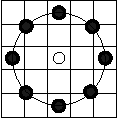
\includegraphics[scale=2.0]{graphics/01_podstawy_teoretyczne/lbp-pr-operator.pdf}
	\caption{ Rozszerzony operator LBP z sąsiedztwem $(8, 2)$ \cite{HEUSCH06} }
	\label{fig:lbp-pr-operator}
\end{figure}

Ponadto zauważono, że większość informacji była zawarta w niewielkim podzbiorze wzorców LBP. Wzorce te zostały nazwane wzorcami jednolitymi (\emph{ang. uniform patterns}) i zawierają co najwyżej dwa przejścia z 0 na 1 lub z 1 na 0 dla kolejnych bitów we wzorcu. 

Dla przykładu $11111111$, $00000000$, $10000111$ i $00001110$ są wzorcami jednolitymi. Natomiast $00011011$, $10001101$, $01010101$ i $01001110$ nie są wzorcami jednolitymi. Przykłady wzorców jednolitych znajdują się również na rys. \ref{fig:lbp-uniform-patterns}.

\begin{figure}[h]
	\centering
	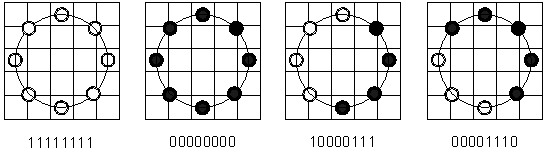
\includegraphics[scale=1.8]{graphics/01_podstawy_teoretyczne/lbp-uniform-patterns.pdf}
	\caption{ Przykładowe 8 bitowe wzorce jednolite }
	\label{fig:lbp-uniform-patterns}
\end{figure}

Nową postać operatora można zapisać jako:
\begin{equation} 
\label{lbp_lbp_riu2} 
LPR_{P, R}^{riu2} = 
	\begin{cases}
		\sum\limits_{p=0}^{P-1} s(g_p - g_c) & \text{ jeżeli } U(LBP_{P, R}) \leq 2 \\
		P + 1 & \text{ jeżeli } U(LBP_{P, R}) > 2
	\end{cases}
\end{equation} gdzie: \begin{equation} 
\label{lbp_u_lbp} 
U(LBP_{P, R}) = | s(g_{P-1} - g_c) -s(g_0 - g_c) | + \sum\limits_{p=1}^{P-1} | s(g_p - g_c) - s(g_{p-1} - g_c) |
\end{equation}

Ze względu na jego niski koszt obliczeniowy, często wykorzystywany jest do rozwiązywania problemu rozpoznawania twarzy\cite{AHONEN04}\cite{HEUSCH06}\cite{MATURANA09}, wykrywania ruchu\cite{HEIKKILA04}, a także normalizacji obrazów\cite{JUST06}.


\subsection{HOG -- Histograms of Oriented Gradients}

Histogram zorientowanych gradientów (\emph{ang. Histogram of Oriented Gradients, HOG}) został zaproponowany przez Dalala jako jednowymiarowy histogram gradientów orientacji w lokalnych regionach obrazu. Jest odporna na wpływ lokalnych warunków oświetleniowych oraz zmiany geometrii.\cite{YAMAUCHI11}





\section{Klasyfikacja}
%TODO wymienic rozne rodzaje klasyfikatorow
%https://www.youtube.com/watch?v=qdDHp29QVdw
...


\subsection{Klasyfikator według funkcji potencjału}
...
	
\subsection{Klasyfikator statystyczny Bayesa}
...
	
\subsection{Klasyfikator według minimalnej odległości}
...
	
\subsection{Klasyfikator k Najbliższych Sąsiadów}
...

\subsection{Maszyna wektorów wspierających (SVM)}
...
	
\section{Ocena klasyfikatorów}
...

\section{Problemy kategoryzacji}
% entry-level categories
% ???
...
\chapter{Porównanie istniejących rozwiązań}
\chapter{Implementacja}

Silnik kategoryzacyjny został zaimplementowany w języku C++, z użyciem środowiska Visual Studio w wersji 2010 Express, która jest czasowo ograniczona i bezpłatna do zastosowań niekomercyjnych.

\section{Język C++ i Visual Studio}

Język C++ jest językiem programowania ogólnego przeznaczenia. Jest językiem wieloparadygmatowym, czyli umożliwia stosowanie różnych paradygmatów programowania: proceduralnego, obiektowego i generycznego. Został zaprojektowany przez Bjarne Stroustrupa jako rozszerzenie języka C i użyty po raz pierwszy w 1979 roku. Charakteryzuje się obiektowymi mechanizmami abstrakcji danych oraz silną statyczną kontrolą typów.

Początkowo do realizacji zadania miał zostać wykorzystany język Python, ze względu na bogactwo bibliotek do uczenia maszynowego oraz przetwarzania obrazów. Warto wspomnieć szczególnie o dwóch bibliotekach: scikit-learn oraz scikit-image, które pozwalają na rozwiązanie wielu problemów związanych z klasyfikacją obrazów, klastrowaniem lub ekstrakcją cech. Zdecydowano o użyciu języka C++ z dwóch powodów:

\begin{compactitem}
	\item \emph{szybkość działania} -- kod jest kompilowany do kodu maszynowego, natomiast Python jest językiem interpretowanym i przez to czas potrzebny na osiągnięcie podobnych wyników jest większy
	\item \emph{silne typowanie} -- w przeciwieństwie do Pythona, język C++ jest silnie typowany, co w ocenie autora niniejszej pracy ma wpływ na zachowanie porządku w kodzie źródłowym
\end{compactitem}

Microsoft Visual Studio jest zintegrowanym środowiskiem programistycznym rozwijanym przez firmę Microsoft. W skład pakietu wchodzą kompilatory kilku języków: C$\sharp$, J$\sharp$, Visual Basic, F$\sharp$, C++ oraz zintegrowany debugger, który działa na poziomie kodu źródłowego, jak i maszyny. Pierwsze wydanie pakietu pojawiło się w 1995 i obecnie najnowszą wersją jest wersja 12 z 2013 roku. 

Kompilator Visual C++ wchodzący w skład pakietu jest specjalną wersją kompilatora języka C++, dostosowana do systemu Windows. Z tego powodu zawiera wiele dedykowanych bibliotek dla tego systemu operacyjnego, które nie mają swoich odpowiednikach w systemach Linux, Unix lub Mac OS X. Dodatkowo Microsoft wydając ten kompilator stworzył swój własny standard języka, który do wersji Visual Studio 2013 nie był w pełni zgodny z ISO. Co za tym idzie, kod silnika powstały w wersji Visual Studio 2010 nie musi być zgodny z ISO.

\section{OpenCV}

Do ekstrakcji cech oraz do klasyfikacji wykorzystano OpenCV. Jest to biblioteka do przetwarzania obrazów napisana w języku C, oparta na otwartym kodzie i zapoczątkowana przez firmę Intel. Charakteryzuje się wieloplatformowością, gdyż istnieją wersje na systemy operacyjne Windows, Mac OS X oraz Linux. Umożliwia ponadto, dzięki zastosowaniu odpowiednich nakładek, na tworzenie kodu w różnych językach programowania: C++, C$\sharp$ oraz Python.


\section{Architektura systemu}
...

\section{Opis API}
...
\chapter{Interpretacja wyników}

W celu określenia jakości działania silnika kategoryzacyjnego przeprowadzono kilka testów. Testy polegały na przeprowadzeniu kategoryzacji obrazów pochodzących ze zbioru Caltech-101.\cite{CALTECH101}

Caltech-101 jest zbiorem obrazów przygotowanych na Kalifornijskim Uniwersytecie Technicznym (w skrócie \emph{Caltech}) przez Fei-Fei Li, Marca Andreetto oraz Marca Aurelio Ranzato. Zawiera obrazy nieobciążone ograniczeniami licencyjnymi podzielone na 101 kategorii.

Obrazy zostały podzielone na zbiory treningowe i testowe w stosunku 50\% na 50\%. Testy zostały przeprowadzone dla 2, 4 oraz 8 kategorii, dla zbiorów treningowych zawierających 1, 5, 10, 15, 20, 30 oraz 40 obrazów na kategorię. Do klasyfikacji wykorzystano rodzaj maszyny wektorów nośnych o nazwie C-Support Vector Classification. Jest to implementacja pozwalająca na klasyfikację n klas i~przyjmuje następujące parametry:

\begin{compactitem}
	\item $C$ -- współczynnik kary, zbyt małe wartości tego parametru skutkują większą ilością błędów podczas trenowania klasyfikatora, co prowadzi do niedostatecznego dopasowania (\emph{underfitting}), zbyt duże wartości skutkują nadmiernym dopasowaniem (\emph{overfitting}),
	\item $\gamma$ -- parametr określa jak duży wpływ na proces klasyfikacji ma pojedynczy przykład.
\end{compactitem}

Właściwy dobór parametrów jest kluczowy do osiągnięcia bardzo dobrych wyników. Na potrzeby testów przyjęto następujące wartości parametrów: $C = 312.5$, $\gamma = 0.50625$.

Poniżej znajdują się wykresy trafności dla poszczególnych przypadków. Liczbę klastrów ustalono na 1500. Kategorie testowe były następujące: samoloty, samochody, lampart, motocykle, budda, żyrandol, pianino. 

\begin{figure}[h]
	\centering
	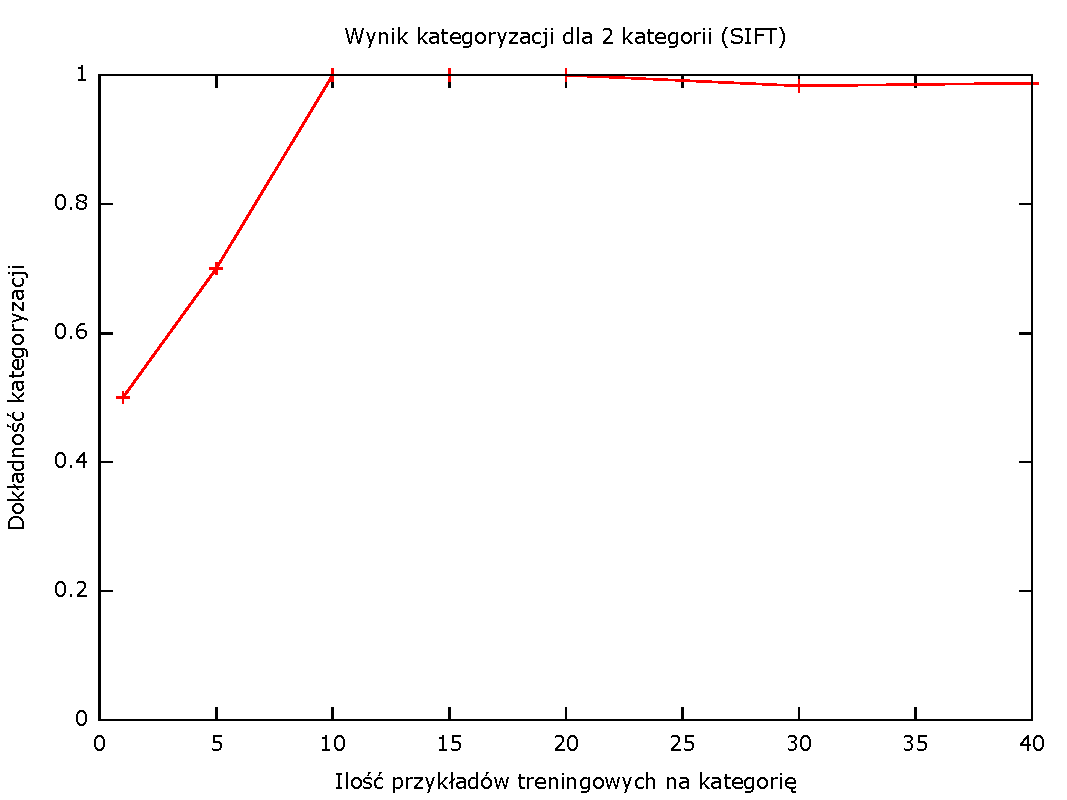
\includegraphics[scale=0.8]{graphics/04_interpretacja_wynikow/result-sift-2.pdf}
	\caption{ Wykres trafności dla uczenia 2 kategorii (SIFT), k=1500 }
	\label{fig:result-sift-2}
\end{figure}

\begin{figure}[h]
	\centering
	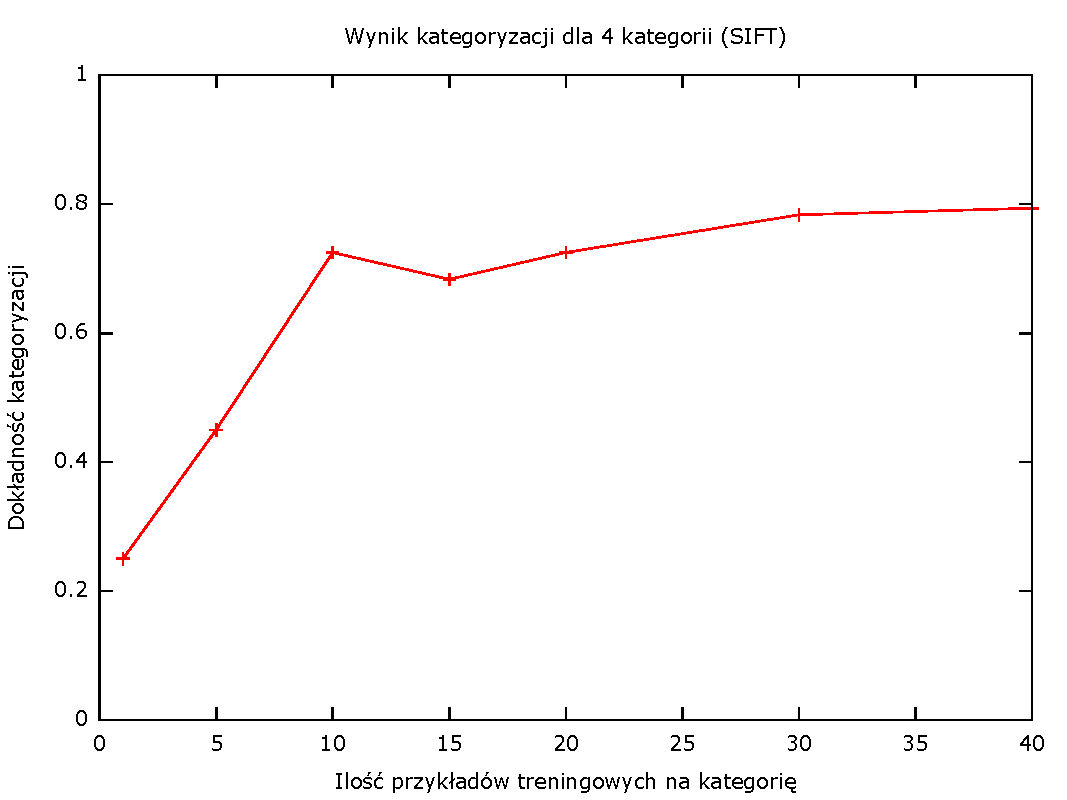
\includegraphics[scale=0.8]{graphics/04_interpretacja_wynikow/result-sift-4.pdf}
	\caption{ Wykres trafności dla uczenia 4 kategorii (SIFT), k=1500 }
	\label{fig:result-sift-4}
\end{figure}

\begin{figure}[h]
	\centering
	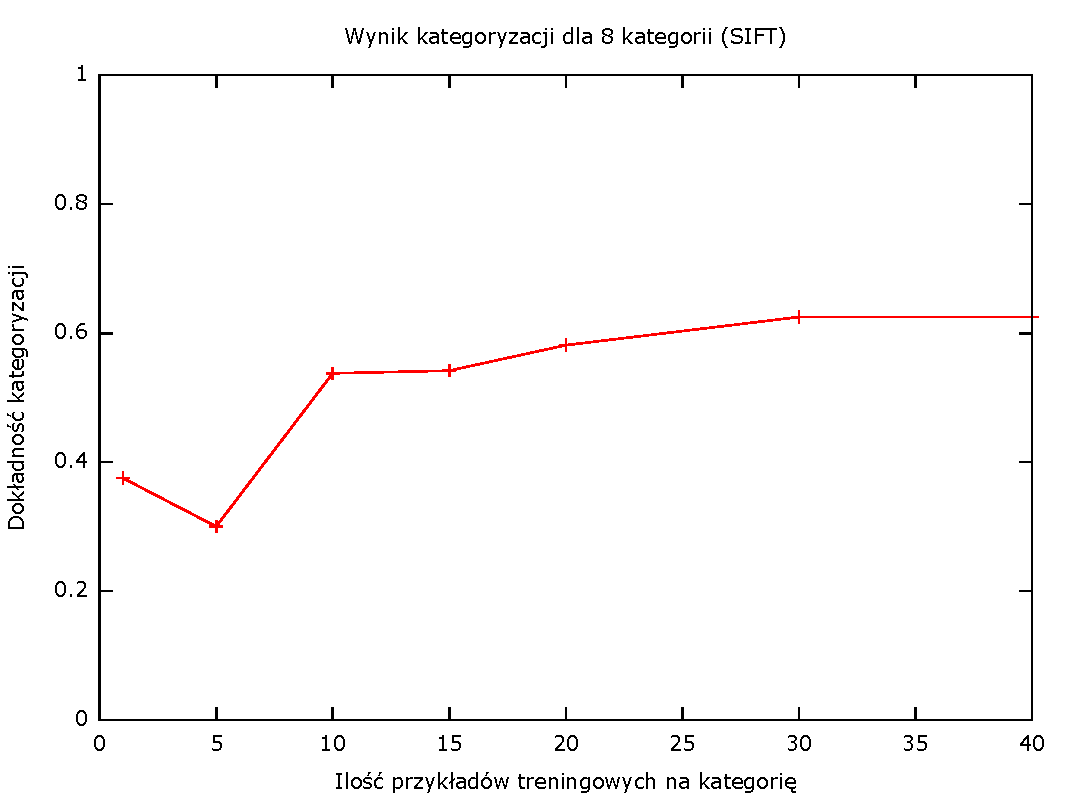
\includegraphics[scale=0.8]{graphics/04_interpretacja_wynikow/result-sift-8.pdf}
	\caption{ Wykres trafności dla uczenia 8 kategorii (SIFT), k=1500 }
	\label{fig:result-sift-8}
\end{figure}

\begin{figure}[h]
	\centering
	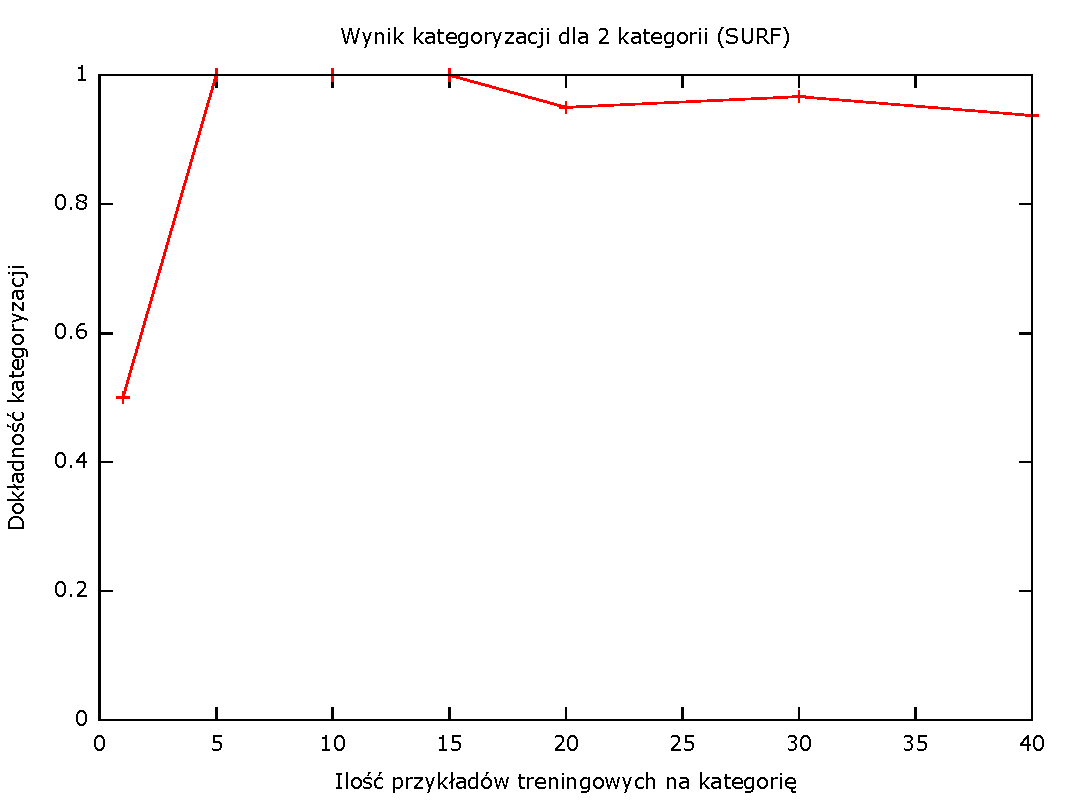
\includegraphics[scale=0.8]{graphics/04_interpretacja_wynikow/result-surf-2.pdf}
	\caption{ Wykres trafności dla uczenia 2 kategorii (SURF), k=1500 }
	\label{fig:result-surf-2}
\end{figure}

\begin{figure}[h]
	\centering
	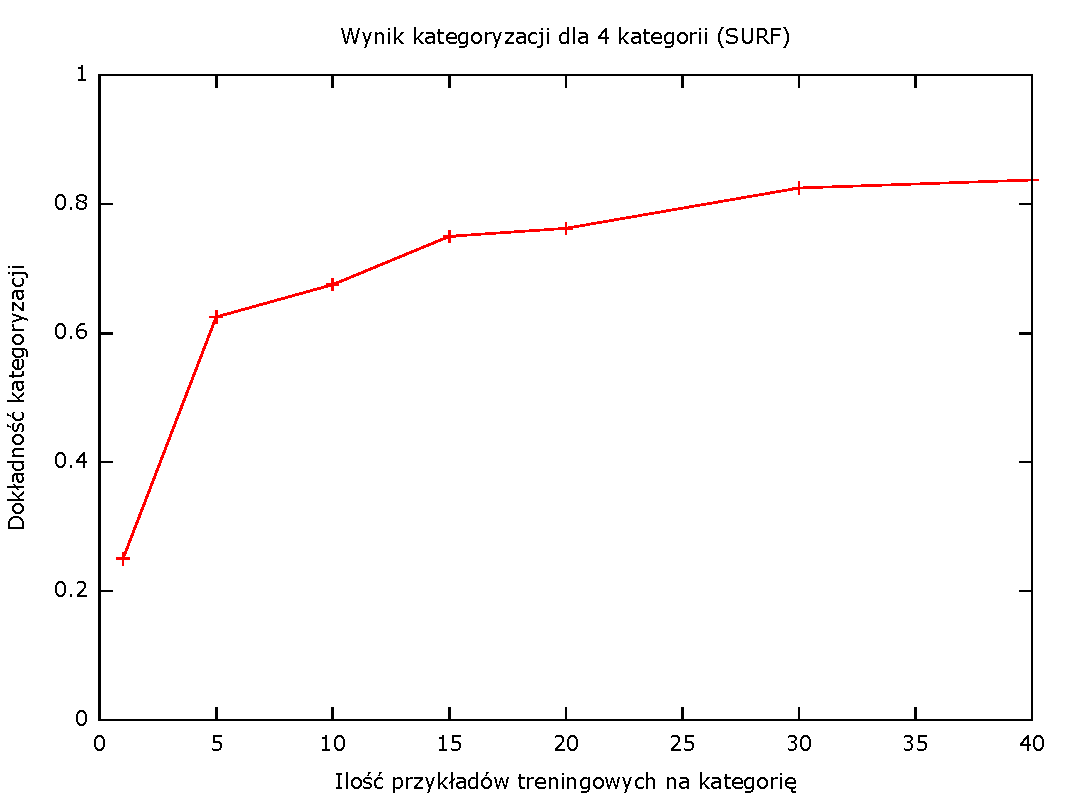
\includegraphics[scale=0.8]{graphics/04_interpretacja_wynikow/result-surf-4.pdf}
	\caption{ Wykres trafności dla uczenia 4 kategorii (SURF), k=1500 }
	\label{fig:result-surf-4}
\end{figure}

\begin{figure}[h]
	\centering
	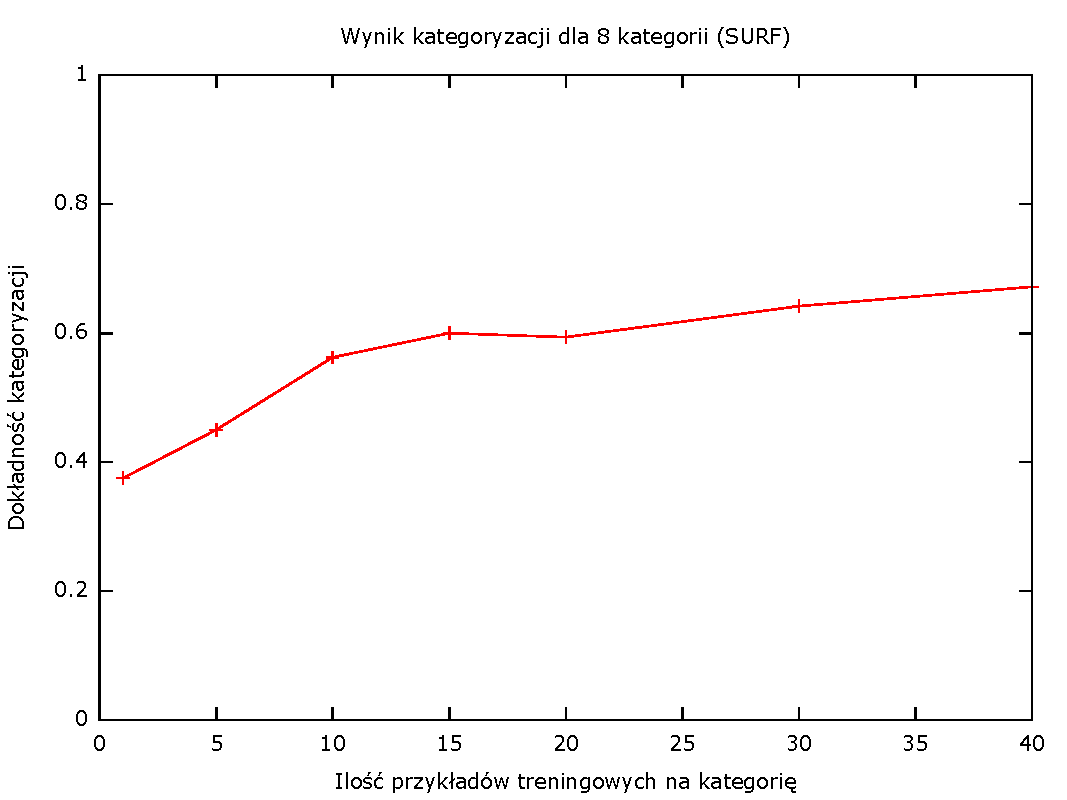
\includegraphics[scale=0.8]{graphics/04_interpretacja_wynikow/result-surf-8.pdf}
	\caption{ Wykres trafności dla uczenia 8 kategorii (SURF), k=1500 }
	\label{fig:result-surf-8}
\end{figure}

Wyniki dla algorytmów SURF i SIFT są zbliżone, jednakże dużo większa czasochłonność algorytmu SIFT jest zauważalna. Widać przewagę SIFT nad SURF w przypadku kategoryzacji dla 2 kategorii. Dokładności dla 2 oraz 4 kategorii są bardzo dobre: odpowiednio ok 90\% i ok. 80\% dla zbiorów treningowych o czterdziestu elementach. Zauważalny jest spadek dokładności dla przypadku 8 kategorii, najlepszy wynik dla tego przypadku wyniósł 67.19\%. 

Dla przypadków 4 i 8 kategorii widoczny jest wzrost dokładności wraz ze wzrostem przykładów w zbiorze uczącym. Dla przypadku 2 kategorii doszło najprawdopodobniej do zjawiska zbytniego dopasowania klasyfikatora, ponieważ do pewnego momentu klasyfikator daje dobre rezultaty, a potem wraz ze wzrostem ilości przykładów, dokładność maleje.

Niezbyt dobre wyniki dla przypadku 8 kategorii mogły być związane z niewłaściwym doborem parametrów, dlatego postanowiono zmniejszyć liczbę klastrów do 500 i przeprowadzono ponowny test dla deskryptora SURF (rys. \ref{fig:result-surf-2-1500-500}, \ref{fig:result-surf-4-1500-500}, \ref{fig:result-surf-8-1500-500}).

\begin{figure}[h]
	\centering
	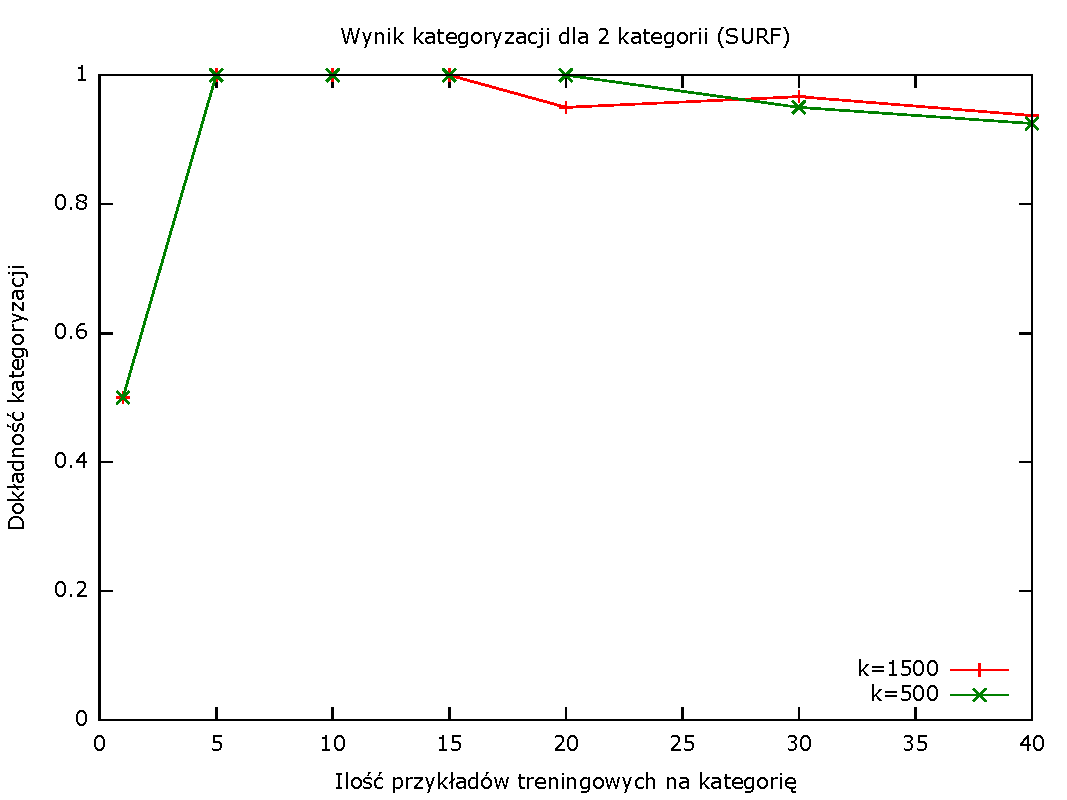
\includegraphics[scale=0.8]{graphics/04_interpretacja_wynikow/result-surf-2-1500-500.pdf}
	\caption{ Wykres trafności dla uczenia 2 kategorii (SURF), k=1500, k=500 }
	\label{fig:result-surf-2-1500-500}
\end{figure}

\begin{figure}[h]
	\centering
	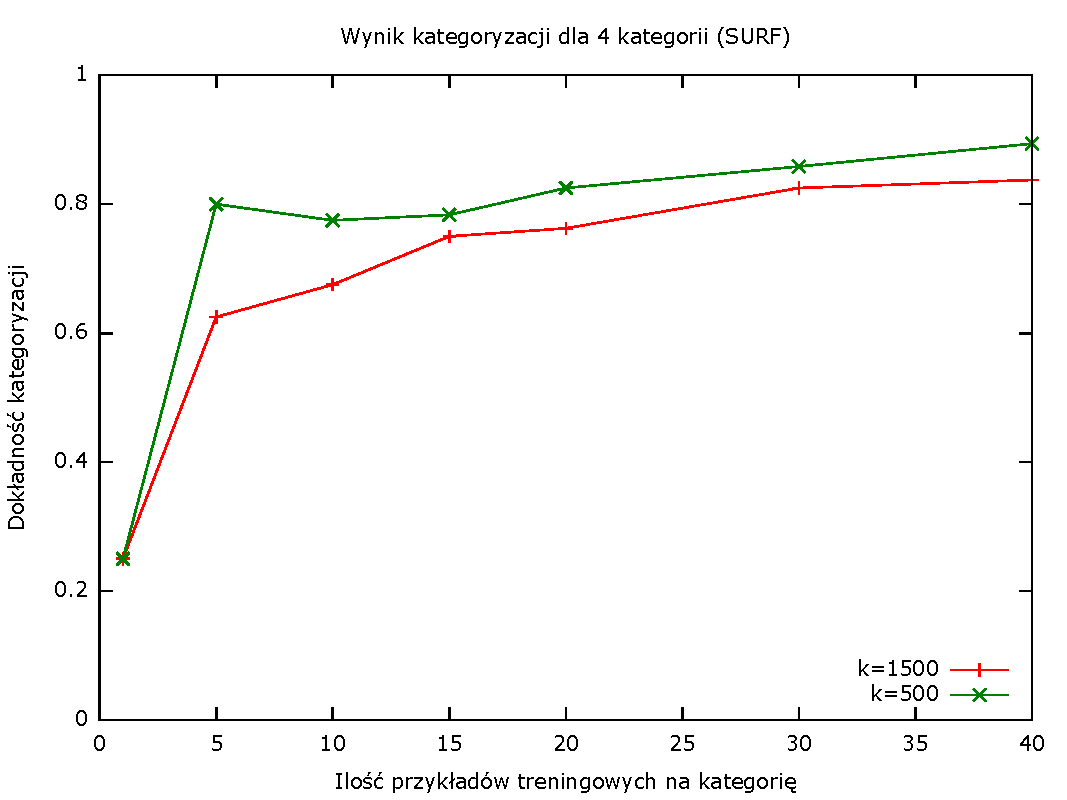
\includegraphics[scale=0.8]{graphics/04_interpretacja_wynikow/result-surf-4-1500-500.pdf}
	\caption{ Wykres trafności dla uczenia 4 kategorii (SURF), k=1500, k=500 }
	\label{fig:result-surf-4-1500-500}
\end{figure}

\begin{figure}[h]
	\centering
	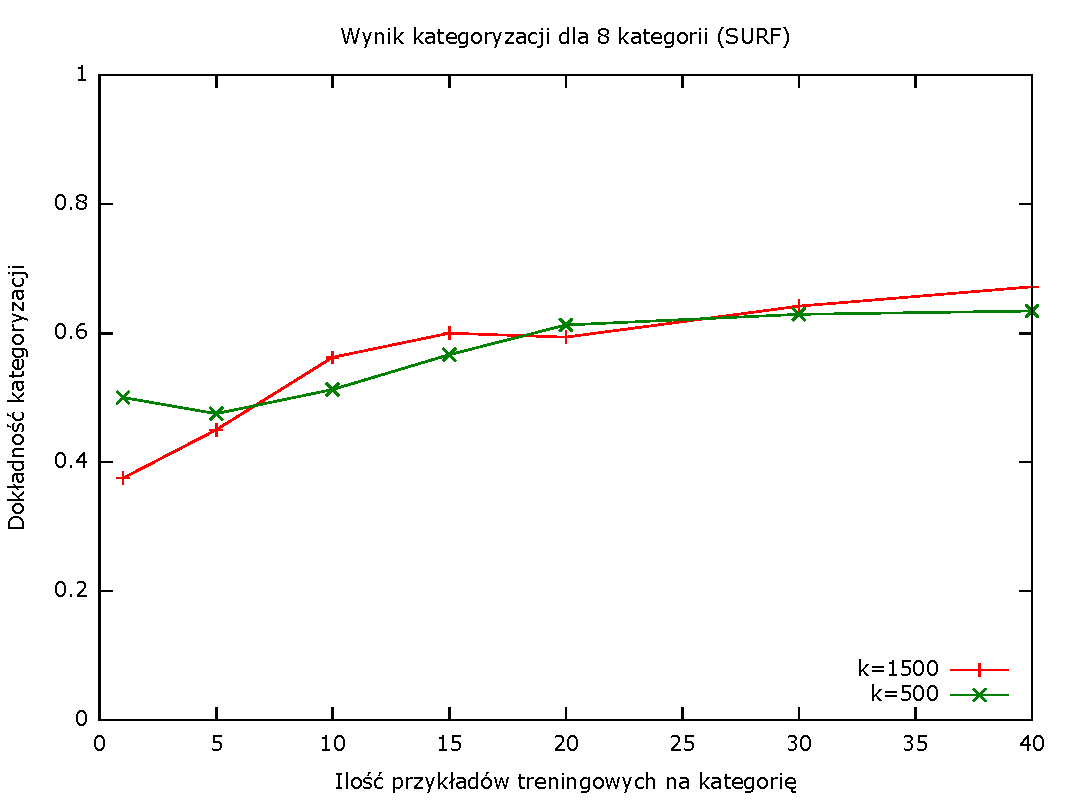
\includegraphics[scale=0.8]{graphics/04_interpretacja_wynikow/result-surf-8-1500-500.pdf}
	\caption{ Wykres trafności dla uczenia 8 kategorii (SURF), k=1500, k=500 }
	\label{fig:result-surf-8-1500-500}
\end{figure}

Zauważono znaczną poprawę dla przypadku 4 kategorii, niestety nie udało się poprawić wyniku dla 8 kategorii, co może wynikać ze zbyt małej liczności zbioru treningowego. Najprawdopodobniej lepsze wyniki można byłoby osiągnąć dla większej liczny przykładów. Większa ilość przykładów powinna skutkować zwiększeniem ilości słów, co za tym idzie należałoby uwzględnić korektę parametrów takich jak $C$ oraz ilość klastrów $k$.
\chapter{Podsumowanie i zakończenie}

Różnorodność technik służących zarówno do ekstrakcji cech obrazów jak i klasyfikacji oraz dostępność dobrze udokumentowanych i zarazem darmowych bibliotek do przetwarzania obrazów pozwala na budowanie coraz skuteczniejszych narzędzi służących do kategoryzacji obrazów. Narzędzia te mogą być bardzo przydatne nie tylko do zapanowania nad zbiorami zdjęć, ale także mogą się przydać do budowy systemów zaawansowanego wyszukiwania grafiki na podstawie zapytań lub do szczegółowej analizy przeglądanych zdjęć w Internecie.

Narzędzie do kategoryzacji zdjęć zaproponowane w niniejszej pracy zostało oparte na metodzie \emph{Bag of Visual Words} i daje bardzo dobre wyniki dla 2 lub 4 kategorii. Wyniki przeprowadzonych testów pozwalają mieć nadzieję na to, że skuteczność metody dla przypadku większej ilości kategorii można poprawić poprzez dostrojenie parametrów maszyny wektorów nośnych oraz powiększenie zbiorów treningowych.



\section{Możliwe dalsze kierunki rozwoju}



\addcontentsline{toc}{chapter}{Bibliografia}
%%%%%%%%%%% Bibliografia %%%%%%%%%%%%%%%%%%%%%%%%%% 
\begin{thebibliography}{100} % 100 is a random guess of the total number of 
%references 

\bibitem{MARKETING12} Baier D., Daniel I., Frost S., \emph{Image data analysis and classification in marketing}, Advances in Data Analysis and Classification , Volume 6, Issue 4 , December 2012, Pages 253-276, ISSN 1862-5347

\bibitem{BISHOP06} Bishop C. M., \emph{Pattern Recognition and Machine Learning}, New York: Springer, 2006, ISBN 0-387-31073-8

\bibitem{CASEY} Casey C., \emph{Part Two: Like it or Not, Predictive Coding is Here and Judges Want you to Use it}, Hudson Legal Blog, 2012, http://us.hudson.com/legal/blog/postid/537/part-2 [dostep: 26.08.2014]

\bibitem{CICHOSZ00} Cichosz P., \emph{Systemy uczące się}, Warszawa: Wydawnictwo Naukowo-Techniczne, 2000, ISBN 83-204-2544-1

\bibitem{GIST09} Douze M., Jégou H., Sandhawalia H., Amsaleg L, Schmid C.,\emph{Evaluation of GIST descriptors for web-scale image search}, Proceedings of the ACM International Conference on Image and Video Retrieval (CIVR '09). ACM, New York, 2009


\bibitem{GLAZER08} Glazer A., Sipper M., \emph{Evolving an Automatic Defect Classification Tool}, Applications of Evolutionary Computing, Heidelberg: Springer, 2008, Pages 194-203

\bibitem{GONZALES01} Gonzales R. C., Woods R. E., \emph{Digital Image Processing}, Boston MA, USA: Addison-Wesley Longman Publishing, 2001, ISBN 0201180758

\bibitem{GMM10} Górriz J. M., Segovia F., Ramírez J., Lassl A., Salas-Gonzalez D., \emph{GMM based SPECT image classification for the diagnosis of Alzheimer’s disease}, Applied Soft Computing, Volume 11, Issue 2, March 2011, Pages 2313-2325, ISSN 1568-4946

%TODO niecytowane
%\bibitem{HMS01} Hand D., Mannila H. Smyth P., \emph{Eksploracja danych}, Warszawa: Wydawnictwo Naukowo-Techniczne, 2005, ISBN 83-204-3053-4

\bibitem{IMAGGA} Imagga APIs Documentation, http://docs.imagga.apiary.io/ [dostęp: 12.08.2014]

\bibitem{LZLM06} Liu Y., Zhang D., Lu G., Ma W-Y., \emph{A survey of content-based image retrieval with high-level semantics}, Pattern Recognition, Volume 40, Issue 1, January 2007, Pages 262-282, ISSN 0031-3203

\bibitem{MONTEJO13} Montejo L.D., Jia J., Kim H. K., Netz U. J., Blaschke S., Müller G. A., Hielscher A. H., \emph{Computer-aided diagnosis of rheumatoid arthritis with optical tomography, Part 2: image classification}, Journal of biomedical optics, Volume 18, Jul 2013, ISSN 1560-2281

\bibitem{MOTODA98} Liu H., Motoda H., \emph{Feature Selection for Knowledge Discovery Data Mining}, Boston: Kluwer Academic Publishers, 1998

\bibitem{SIFT99} Lowe D. G., \emph{Object Recognition from Local Scale-Invariant Features}, Proceedings of the International Conference on Computer Vision-Volume 2 - Volume 2 (ICCV '99), Vol. 2. IEEE Computer Society, 1999, Page 1150

\bibitem{PIXIT} PiXiT, http://www.montefiore.ulg.ac.be/~maree/pixit.html [dostęp: 12.08.2014]

\bibitem{Google2010} Smith N., \emph{Ooh! Ahh! Google Images presents a nicer way to surf the visual web}, Google Official Blog, 2010, http://googleblog.blogspot.com/2010/07/ooh-ahh-google-images-presents-nicer.html [dostęp: 05.08.2014]

\bibitem{STRUMIL} Strumillo P., \emph{Przetwarzanie obrazów, wykłady}, http://www.eletel.p.lodz.pl/pstrumil/ [dostęp: 6.09.2014]

\bibitem{SUVDAA2012} Suvdaa B., Ahn J., Ko J., \emph{Steel Surface Defects Detection and Classification Using SIFT and Voting Strategy}, International Journal of Software Engineering and Its Applications, Volume 6, No. 2, Apri 2012, Pages 161-166

\bibitem{Tad91} Tadeusiewicz R., Flasiński M., \emph{Rozpoznawanie obrazów}, Warszawa: Państwowe Wydawnictwo Naukowe, 1991, ISBN 83-01-10558-5

\bibitem{WARWICK10} Wernick M.N., Yongyi Y., Brankov J.G., Yourganov G., Strother S.C., \emph{Machine Learning in Medical Imaging}, Signal Processing Magazine, IEEE, Volume 27,  Issue 4, July 2010, Pages 25-38

\bibitem{VALPOLA} Valpola H., \emph{Bayesian Ensemble Learning for Nonlinear Factor Analysis}, Acta Polytechnica Scandinavica, Mathematics and Computing Series No. 108, Espoo 2000, 54 pp.
 
\end{thebibliography} 
%%%%%%%%%%%%% end %%%%%%%%%%%%%%%%%%%%%%%%%%%%%%% 
\end{document}
